\documentclass[]{vgtuef}
\usepackage[utf8x]{inputenc}
\usepackage[L7x]{fontenc}
\usepackage[lithuanian]{babel}

\author{Maksim Norkin\\Vilniaus Gedimino technikos
  universitetas\\Elektronikos fakultetas\\Elektroninių sistemų
  katedra\\\texttt{maksim.norkin@ieee.org}}
\title{Bakalauro baigiamasis darbas\\Parkinsono ligos eigos stebėjimo priemonė}


\begin{document}

\setcounter{page}{7}

\onehalfspacing

\layout

\tableofcontents

\section*{Žymenys ir santrumpos}
\addcontentsline{toc}{section}{Žymenys ir santrumpos}

\begin{itemize}
\item VŽRJ - Vertikali žemės reakcijos jėga (angl. Vertical Ground Reaction Force);
\item PCA - principinė komponenčių analizė (angl. Principal Component Analysis);
\item LDA - linijinė disktriminanto analizė (angl. Linear Diskriminant Analysis);
\item Co - kontrolinis subjektas, kurio ligos istorijoje nebuvo užregistruota jokių neurologinių susirgimų;
\item Pt - Parkinsono liga sergantis subjektas;
\end{itemize}

\section{Įvadas. Užduoties analizė}

Darbo tema yra Parkinsono ligos eigos stebėjimo programa. Parkinsono liga yra dažniausiai pasitaikantis neurodegeneracinis judėjimo sutrikimas. Ankstyva ligos diagnozė ir efektyvus terapijos terapijos stebėjimas yra būtinas pacientų gydymui ir sveikatos priežiūros kainai sumažinti. Šiuo metu neegzistuoja gydytojų patvirtintos objektyvios ir vieningos vertinimo sistemos, kuri tiksliai atpažintų Parkinsono ligos simptomus. Vienas iš didžiausiai pasireiškiančių simptomų yra eisenos sutrikimas. Sutrikimo dažnumą ir svarbą patvirtina ir viešai prieinama duomenų bazė, kurioje yra pateikiami sveikų ir sergančių Parinsono liga žmonių eisenos duomenys. Duomenų bazė vadinasi ``PhysioBank'' \cite{932728}.

Darbo tikslas yra sukurti programą, gebančią atpažinti jėgos jutikliais gautus signalus, priklausančius Parkinsono liga sergantiems subjektams. Programa bus įgyvendinta Matlab platformoje. Tokia platforma buvo pasirinkta dėl plataus įrankių kiekio, kuris yra prieinamas Matlab aplinkoje. Taip pat nurodytoje platformoje yra labai patogu ir greita realizuoti signalų apdorojimo sistemas dėl architektūros - visi kintamieji yra matricos. 

Darbe bus panaudoti duomenis, kuriuos pateikia jėgos jutikliai. Jie matuoja vertikalią žemės reakcijos jėga (VŽRJ) (angl. Vertical Ground Reaction Force (vGRF)). Fizikoje, ir būtent biomechanikoje, VŽRJ nurodo kokia jėga žemė atsako ją slegiančiam objektui. Kaip pavyzdžiui, stovinti žmogus slegia žemę jėga, kuri lygi jo masei ir tuo pat metu, žemė slegia žmogų priešinga, lygiai tokia pačia jėga. Tokie jutikliai buvo parinkti dėl to, kad šaltiniai \cite{S0966-6362(05)00058-5} nurodo VŽRJ kaip žmogaus kūno stabilumo indikatorių.

Parkinsono liga buvo pasirinkta dėl to, kad šiuo metu ji yra aktyviai tiriama \cite{vgtu}, kadangi visuomenė moka labai didelius pinigus Parkinsono liga sergantiems asmenims. Per metus ši suma gali siekti 6 milijardus dolerių. Ligos rizika su amžiumi tik didėja, todėl analitikai prognozuoja, kad ateityje visuomenė mokės žymiai daugiau dėl žmonių populiacijos senėjimo.

Didžiausia ligos atpažinimo problema slypi savybių, kurios geriausiai atskirs sergantį Parkinsono liga nuo sveiko, nesergančio asmens. Darbo metu bus apžvelgtos kelios galimo savybės, kurios gali atskirti tokius subjektus. Blogiausias galimas variantas būtų nelinijinė funkcija atskirti didelių dimensijų duomenys. Geriausias galimas variantas būtų mažos dimensijos duomenys (iki 3 dimensijų) ir linijiškai atskiriami duomenys (kadangi linijinę funkciją realizuoti yra lengviausia). Turint didelių dimensijų duomenis, planuojamos sistemos aparatiniai reikalavimai automatiškai padidėja, kadangi būtina apdoroji labai daug duomenų. Tokią problemą galima išspręsti panaudojus dimensijų mažinimo algoritmus, kurių dažniausiai taikomi \cite{824819}: Principinių komponenčių analizė (angl. Principal Component Analysis (PCA)), linijinė diskriminanto analizė (anl. Linear Discriminant Analysis (LDA)). Metodai bus aptarti vėlesnėse skyriuose. Jie taip pat vadinami dimensijų praskyrimo algoritmai. Jie yra taikomi, kuomet duomenis yra atskirti netiesiškai. Duomenims, atskirtu tiesiniu dėsniu, galima taikyti paprastą klasifikavimo algoritmą. Jeigu duomenis taip ir nepavyksta atskirti tiesiškai, tenka taikyti kompleksinį klasifikatorių, ko pasekoje gali labai sumažėti klasifikavimo rezultatas. Darbe bus panaudotas Matlab aplinkoje įgyvendintas įrankis, kuris skirtas suprojektuoti naują dimensijų plokštumą, kurį įgyvendino Vojtech Franc savo magistriniam darbe \cite{stprtool}. Darbas buvo apgintas 2000 metais, Čekijos technikos universitete, Prahoje. Tiesinio sklidimo dirbtinių neuronų klasifikatorių bus panaudotas iš Matlab ``Neural Network Toolbox'' įrankio. Likusi sistemos dalis bus aprašyta šiame darbe.

Sukurtas produktas gebės pateikti diagnozę - ar subjektas turi Parkinsono liga sergančių subjektų eisenos požymių ar jų neturi. Produktas neatsižvelgs į kitus ligos simptomus: drebulys (rankų, kojų, žandikaulio, galvos), standumas (galūnių arba liemens sustingimas), bradikinezija (judesių lėtumas), pozicijos nestabilumas (arba sutrikęs balansas). Pati programa duomenis analizuos jau po duomenų surinkimo. Tai reiškia, kad pirmiausiai duomenys bus surenkami, o vėliau įkeliami į programą tolimesniam apdorojimui.

Darbo tema, Parkinsono ligos eigos stebėjimo programa, reiškia, darbo rezultate bus sukurtas algoritmas, kuriuo bus parengta kompiuterinė programa. Pačiam kompiuteryje turi būti veikiantis Matlab programinis paketas. Programa bus rašoma Matlab 7.12.0 (R2011) versija su ``Neural Network Toolbox'' įrankiu. Eigos stebėjimas reiškia, kad visuomet egzistuoja neapibrėžtas, galimas programos netikslumas. Visiškai programa remtis, diagnozuojant Parkinsono ligą nėra galima, kadangi, kaip jau buvo minėta ankščiau - eigos sutrikimas nėra vienintelis ligos požymis. Turi būti atlikti ir kiti tyrimai, norint tiksliai diagnozuoti ligą.

Darbo objekto sudėtis yra asmeniniam kompiuteriui skirta programa, jėgos jutiklių signalų generavimo programa. Kokiam kompiuteriui programa bus rašoma, paminėta ankščiau. Jėgos jutiklių generavimo programa (modulis) bus atsakinga už signalų nuskaitymą iš duomenų bazės ir jų pateikimą sistemos algoritmui. Taip pat signalų generavimo programa (modulis) bus naudojamas programos demonstracinei versijai įgyvendinti.

Kaip buvo minėta, duomenys sistemai bus pateikiami iš ``PhysioBank'' duomenų bazės \cite{932728}. Duomenys duomenų bazėje buvo surinkti diskretizuojant signalus $100~Hz$ diskretizavimo dažniu. Kiekvienu laiko momentu, yra įrašoma nauja eilutė į duomenų tekstinę bylą. Eilutę sudaro 19 skilčių:

\begin{itemize}
\item Skiltis 1 nurodo laiką (sekundėmis);
\item Skiltys 2-9 nurodo kairės kojos 8 jutiklių VŽRJ, Niutonais;
\item Skiltys 10-17 nurodo dešinės kojos 8 jutiklių VŽRJ, Niutonais;
\item Skiltis 18 nurodo kairės kojos suminę VŽRJ, Niutonais;
\item Skiltis 19 nurodo dešinės kojos suminę VŽRJ, Niutonais;
\end{itemize}

Duomenų bazės bylų pavadinimai, pavyzdžiui: ``GaCo01\_02.txt'' ar ``JuPt03\_06.txt'', sudaryti nurodant duomenų rinkimų sesijų pavadinimus: ``Ga'' - ``Galit Yogev et al'' (dual tasking in PD; Eur J Neuro, 2005), ``Ju'' - ``Hausdoff et al'' (RAS in PD; Eur J Neuro, 2007), ``Si'' - ``Silvi Frenkel-Toledo et al'' (Treadmill walking in PD; Mov Disorders, 2005). Toliau, ``Co'' nurodo kontrolinį subjektą arba nesergantį Parinsono liga subjektą, ``Pt'' nurodo Parkinsonu sergantį subjektą. Pirmas numeris nurodo subjekto identifikacinį numerį, po brūkšnio einantis antras numeris nurodo subjekto duomenų rinkimo seką. Aprašyme nurodyta, kad visuose duomenų rinkimų sesijose iš viso dalyvavo $93$ sergantis subjektas ir $73$ Parkinsono liga sergantis subjektas.

Programos veikimas bus vertinamas taiklumu ir jautrumu. Parametrai yra apskaičiuojami iš pasikliovimo matricos.

\section{Informacinių Parkinsono ligos diagnostikos sistemų apžvalga}

Šiame skyriuje bus apžvelgtos analoginės informacinės sistemos arba bandymai sukurti sistemą, kuri, remiantis įvairių jutiklių pagalba, gebėtų atpažinti Parkinsono ligą. Apibendrintai bus aptarti nagrinėjamų sistemų teigiamos ir neigiamos savybės - ar pasirinkti požymiai yra argumentuoti ar naudojamas klasifikatorius yra parinktas atsižvelgus į naudojamą savybių erdvę.

%% PIRMAS DARBAS

Pirmas darbas, kuris bus apžvelgtas yra ``Statistical Analysis of Gait Rhythm in Patients With Parkinson's Disease'' \cite{5280353}. Šis darbas nagrinėja galimas žingsnio variacijos galimybes ir pateikia signalo nuokrypio skaičiavimą kaip pagrindinę savybę, atskiriančia kontrolinius subjektus nuo sergančių. Nagrinėjime buvo panaudoti žingsnio pakilimo nuo žemės ilgis, žingsnio prisilietimo prie žemės ilgis ir bendras žingsnio ilgis. Duomenys gaunami, iš vertikalią žemės reakcijos jėgos matavimų. Autorių teigimu, žingsnio pakilimo ir nusileidimo ilgiai turi aukštą koreliacijos koeficientą su bendro žingsnio ilgiu, todėl nagrinėjime buvo panaudotas tik bendro žingsnio ilgis (\ref{table:stance_swing_string_corr} lentelė). Gautas savybių vektorius buvo apskaičiuotas, naudojantis ``vieno palikimo-išmetimo tarpusavio patikros'' (angl. leave-one-out cross-validation) metodu. Jis parodė, kad mažiausių šaknų vektoriaus palaikymo mašina (angl. Support Vector Machine), su polinominiu branduoliu sugeba klasifikuoti duomenis su $90.32 \%$ tikslumu. 

Nagrinėjime buvo naudoti duomenis, pateikti ``Hausdorff et al'' \cite{MDS:MDS870130310}, kurie yra  laisvai prieinami iš PhysioNet duomenų bazės \cite{932728}. Tokie duomenys bus panaudoti ir šiame darbe, todėl reikia įsigilinti ir į subjektus, kurie dalyvavo duomenų rinkimo metu. Tyrime dalyvavo 16 sveikų subjektų, 20-74 metų amžiaus. Kontroliniai subjektai buvo visiškai sveiki neurologiškai, neturi jokių širdies ligų sutrikimų. Parkinsono subjektų buvo 15, kurių amžius variavo nuo 44 iki 80 metų. Ūgis ir svoris žymiai nesiskyrė tarp kontrolinių ir Parkinsono subjektų, todėl į tokius duomenis dėmesio nebuvo kreipiama. Parkinsono subjektai buvo vertinami pagal ``Hoehn and Yahr (HAY)'' vertinimo sistemą, nustatant jų ligos stadiją. Du pacientai surinko 1.5 HAY balo (lengva stadija), keturi pacientai surinko tarp 2 ir 2.5 HAY balo, penki surinko 3 HAY balo (vidutinė stadija), likusieji surinko virš 3 HAY balų, jie turėjo žymesnių eisenos sutrikimų. 

\begin{table}[b]
  \renewcommand{\arraystretch}{1.3}
  \centering
  \caption{Koreliacijos koeficientai tarp $\sigma$ bendro žingsnio ($\sigma_r$),
    kojos pakilimo ($\sigma_w$) ir kojos prisilietimo ($\sigma_a$)
    prie žemės ilgio parametrų \cite{5280353}.}
  \label{table:stance_swing_string_corr}
  \begin{tabular}{|c|c|c|c|} \hline
    $\sigma$ & $\sigma_r$ & $\sigma_w$ & $\sigma_a$ \\ \hline
    $\sigma_r$ & 1.00 & 0.99 & 0.94 \\ \hline
    $\sigma_w$ & 0.99 & 1.00 & 0.94 \\ \hline
    $\sigma_a$ & 0.94 & 0.94 & 1.00 \\ \hline
  \end{tabular}
\end{table}

Remiantis gauta pasiskirstymo funkcija, kuri žymima  $\hat{p}(x_b)$, kur $x_b, b = 1, 2, ..., B$, kur $B$ nusako segmentų skaičių, skaičiuojant $x$ amplitudės ruožą, vidurkis $\mu$ ir variacija $\sigma^2$ apskaičiuojama:

\begin{equation}
\mu = \sum_{b=1}^{B} x_b \hat{p}(x_b),
\end{equation}

\begin{equation}
\sigma^2 = \sum_{b=1}^{B} (x_b - \mu)^2 \hat{p}(x_b).
\end{equation}

Tyrimo metu buvo nustatyta, kad Parkinsono subjektų žingsnio ilgio variacija yra žymiai padidėjusi, lyginant su kontroliniais subjektais (\ref{table:gait_corr_params} lentelė), tačiau žingsnio vidurkis lieka beveik nepakitęs. Lentelėje taip pat pateikiami \textit{STC} (angl. Signal Turn Counter) savybės vertės. Signalo $x(i)$ STC skaičiuojamas, remiantis tokiu loginiu ryšiu:

\begin{equation}
 if \left\{ \begin{array}{l}
 	[x(i)-x(i-1)][x(i+1)-x(i)] < 0 \\
 	|x(i+1)-x(i)| \leq Th, 2 \leq i \leq I-1
 \end{array} \right. ,
\end{equation}
kur $Th$ nusako ribinę vertę, $I$ nusako signalo ilgį.

Tokia savybė taip pat turi žymių skirtumų tarp kontrolinio subjekto ir Parkinsono subjekto, tačiau ši savybė turi neigiamą aspektą - jos rezultatas priklauso ne nuo signalo kitimo pobūdžio, o nuo pasirinktos ribinės vertės (toks matematinis procesas dar vadinamas ``derinimu''), o tai neatspindi Parkinsono subjektų eisenos ypatybės. Tokio matematinio ``derinimo'' rezultate gali įvykti, kad algoritmas bus priderintas būtent prie nagrinėjime naudojamų duomenų, tačiau jis gali būti visiškai bevertis į jį pateikus visiškai nematytus algoritmui duomenis.

\begin{table}
  \centering
  \caption{Bendro žingsio, kojos pakilimo, kojos prisilietimo prie žemės vidurkio, vidutinio nuokrypio duomenys \cite{5280353}.}
  \label{table:gait_corr_params}
  \renewcommand{\arraystretch}{1.3}
	\begin{tabular}{|c|c|c|c|} \hline
		 \multirow{2}{*}{Žingsnio fazė} & 
		 \multirow{2}{*}{Statistinis parametras} & Kontrolinis subjektas & Parkinsono subjektas \\ 	\cline{3-4}
		 & & Vidurkis $\pm$ nukrypimas & Vidurkis $\pm$ nukrypimas \\ \hline
		 \multirow{3}{*}{Bendras žingsnis} 
		 	& $\mu(s)$    & $1.09 \pm 0.09$   & $1.12 \pm 0.12$ \\ \cline{2-4}
		 	& $\sigma(s)$ & $0.03 \pm 0.01$   & $0.06 \pm 0.04$ \\ \cline{2-4} 
		 	& $STC$       & $12.44 \pm 10.46$ & $55.87 \pm 29.89$ \\ \hline
		 \multirow{3}{*}{Kojos pakilimas}
	 	 	& $\mu(s)$    & $0.39 \pm 0.04$   & $0.37 \pm 0.05$ \\ \cline{2-4}
		 	& $\sigma(s)$ & $0.02 \pm 0.01$   & $0.04 \pm 0.02$ \\ \cline{2-4} 
		 	& $STC$       & $8.5 \pm 9.39$    & $54.13 \pm 26.96$ \\ \hline
		 \multirow{3}{*}{Kojos prisilietimas}
		 	& $\mu(s)$    & $0.70 \pm 0.06$   & $0.75 \pm 0.09$ \\ \cline{2-4}
		 	& $\sigma(s)$ & $0.02 \pm 0.01$   & $0.05 \pm 0.04$ \\ \cline{2-4} 
		 	& $STC$       & $15.81 \pm 12.07$ & $61.27 \pm 25.62$ \\ \hline
	\end{tabular}
\end{table}

Iš gauto tyrimo rezultato, galima spręsti, kad bendro žingsnio, kojos pakilimo, kojos prisilietimo prie žemės signalo ilgio dispersija ($\sigma$) gali būti panaudoti kaip savybės, norint identifikuoti Parkinsono subjektą.

Sekančiam darbe, kuris bus pateiktas apžvalgai \cite{6091948}, nėra naudojama vertikali žemės reakcijos jėga, skaičiuojant savybes. Sprendimas orientuojamas naudoti pigius, keturis linijinio pagreičio jutiklius. Toks sprendimas yra paprastesnis, už prieš tai apžvelgtą, kadangi jame buvo panaudoti šešiolika vertikalios žemės reakcijos jutiklių. Nagrinėjamos Parkinsono ligos požymiai buvo eisenos stingimas ir nesimetriškumas. Iš pirminės sprendimo apžvalgos iškarto galimas toks sprendimo trūkumas - tiriant galimas savybes, buvo panaudotas tik vienas Parkinsono liga sergantis subjektas ir vienas kontrolinis subjektas. Taip atliekant tyrimą, egzistuoja didelė tikimybė, kad visos gaunamos signalo eisenos savybės gali būti būdingos tik nagrinėjamam subjektui, tačiau gali visiškai negalioti kitiems subjektams ar subjektų grupei. Egzistuoja ir tokia tikimybė, kad ištirtos savybės, kurios galioja Parkinsono subjektui, gali galioti ir kontroliniam subjektui, kadangi buvo panaudotas tik vienas kontrolinis subjektas tyrimo metu.

Nepriklausomai nuo atlikti tyrimo siaurumo, darbe yra pateikta svarbios eisenos analizės išvados. Kontrolinio subjekto eisenoje nebuvo pastebėta jokių eisenos sustingimo požymių, kairės ir dešinės kojos motorinės operacijos buvo atliekamos simetriškai, išskyrus kairės kojos kelio didžiausios amplitudės pagreičio kojos susilietimo ir pakilimo su žeme metu. Abiejų kojų susilietimo su žeme laiko ilgis buvo simetriškas, kas ir patvirtina pusiausvyrą eiseną. Parkinsono subjektas parodė dešinės kojos eisenos sąstingio nesimetriškumą. Pacientas naudojo kompensacijos mechanizmą, kadangi jo eisena automatiškai turėjo stoką. Jis peržengdavo dešinės pusės judesius, kuomet pradėdavo ėjimą. Kairės pusės judesiai buvo atliekami tik palaikant balansą. Pati eisena yra labai lėta, o sustingimas įvyksta tik dešinėje pusėje. Iš gautų rezultatų seka, kad analizuojamas pacientas visuomet bando kompensuoti eisenos pokyti, naudodamasis viena puse. Kadangi tyrimas buvo atliktas tik su vienu pacientu, nėra galima tiksliai nusakyti, kad kompensacija vyksta tik iš dešinės pusės, tačiau ką galima tvirtai sakyti, kad naudojantis kompensacijos mechanizmą - egzistuoja padidėjusi variacijos tikimybę. Tokią hipotezę sėkmingai patvirtina ir prieš tai atlikta darbo analizė \cite{5280353}. Kompensacijos nebuvimas kontrolinio subjekto atveju garantuoja, kad žingsnio ilgio variacija nebus didelė, o atvirkščiai - artės į nulį.

%% ANTRAS DARBAS

Tolimesnė sistema apžvalgai siūlo jau konkretų algoritmą ir techninę įrangą jo įgyvendinimui - ``Characterization of gait abnormalities in Parkinson's disease using a wireless inertial sensor system'' \cite{5627904}. Darbe panaudoti žingsnio, siūbavimo ir nuokrypio sukimo fizinės eisenos savybės ėjimo metu, panaudota principinė komponenčių analizė (angl. Principal Component Analysis (PCA)) savybių erdvės sudarymui ir palaikymo vektorių mašina (angl. support vector machine (SVM)) klasifikavimo mechanizmui įgyvendinti. Naudojama sensorinė Micro-AHRS sensorinė platforma į kurią įeina $50-g$ trijų ašių linijinio pagreičio jutiklis ir $1200~^\circ/s$ trijų ašių kampinio pagreičio jutiklis. Gautas modelis sėkmingai veikia $93~\%$ tikslumu ir taiklumu. Naudojamas svoriui jautrus (angl. cost-sensetive) apmokymas tam, kad nustatyti kokios savybės turi didesnę reikšmę formuojant savybių erdvę, bei atliekant klasifikavimą. Sprendimas buvo atliktas, panaudojus pakankamą skaičių subjektų - 23 subjektai su diagnozuota Parkinsono liga ir 16 kontrolinių subjektų, kurie neturi jokių neurologinių susirgimų ligos istorijoje. Tyrimo metu taip pat buvo nustatytas tikslas identifikuoti mažą ir didelį eisenos sutrikimo atvejį. Iš dalyvaujančių Parkinsono subjektų, 11 turi didelį eisenos sutrikimą, 12 turi mažesnį eisenos sutrikimą. 

Tyrime buvo panaudoti iš viso 67 normalizuotos laiko srities savybės, kurios yra svarbios motorinei veiklai. Duomenys buvo normalizuoti dėl skirtingų savybių amplitudės srities. Normalizacija yra labai svarbi procedūrą, prieš pateikiant duomenis dimensijų analizavimo metodui. Taip yra užtikrinama, kad naudojamos savybės turi vienodą įtakos faktorių, projektuojant naują dimensijų erdvę \cite{824819}. Po dimensijų mažinimo metodo pritaikymo, liko tik 11 savybių, kurių bendra variacija yra $80.20~\%$. Parkinsono ligos eigos sunkumui nustatyti, prie bendros savybių erdvės buvo pridėti dar papildomos keturios savybės. Sprendimas, pateikti klasifikatoriui dar papildomas keturias dimensijas nebuvo tiksliai argumentuotas. Nėra nurodyta ar savybės buvo įterptos po dimensijų mažinimo ar prieš tai. Jeigu tai buvo atlikta po dimensijų mažinimo, tai kelia abejonių naujai sukonstruota erdvė - sistema nėra gerai apibendrinta, jinai yra ``priderinta'' prie esamų duomenų, todėl kelia abejonių ir pačio produkto lankstumas naujų, nematytų duomenų atžvilgiu. 

\begin{table}
	\centering
  \renewcommand{\arraystretch}{1.3}
	\caption{Klasifikavimo rezultatas, naudojant pastovų ir kintantį klaidingo klasifikavimo metodo kriterijų \cite{5627904}.}
	\label{table:wireless_svm_pd_recognition}
	\begin{tabular}{|c|c|c|} \hline
		& Pastovus kriterijus & Kintantis kriterijus \\ \hline
	Jautrumas & $93.3~\%$ & $88.9~\%$ \\ \hline
	Taiklumas & $95.8~\%$ & $100.0~\%$ \\ \hline
	Klaidingai klasifikuotas rodiklis & $4.2~\%$ & $0.0~\%$ \\ \hline
	Tikslumas & $97.7~\%$ & $100.0~\%$ \\ \hline
	\end{tabular}
\end{table}

\begin{table}
	\centering
	\renewcommand{\arraystretch}{1.3}
	\caption{Klasifikavimo rezultatas identifikuojant lengvą ir sunkią Parkinsono ligos eigos atveji. \cite{5627904}.}
	\label{table:wireless_svm_recognition}
	\begin{tabular}{|c|c|c|} \hline
		& Klasės atpažinimas & Klasės tikslumas \\ \hline
	Sunkus PD eisenos sutrikimas & $52.4~\%$ & $84.6~\%$ \\ \hline
	Lengvas PD eisenos sutrikimas & $66.7~\%$ & $64.0~\%$ \\ \hline
	Kontrolinis subjektas & $91.7~\%$ & $71.0~\%$ \\ \hline
	\end{tabular}
\end{table}

Nepaisant neaiškumų dėl savybių erdvės - vektoriaus palaikymo mašinos klasifikatorius su radialiniu gauso branduoliu sugeba subendrinti savybių erdvę. Parkinsono subjekto atpažinimas yra pateiktas \ref{table:wireless_svm_pd_recognition} lentelėje. Geriausias klasifikavimo rezultatas buvo pasiektas, naudojant kintamą klaidos vertinimo kriterijų. Nurodytas klasifikavimo metodas atpažįsta Parkinsono ligą labai gerai ($100~\%$ tikslumas). Toks rezultatas yra labai didelis iššūkis darbe naudojamai sistemai. Projektuojama sistema turi mažiausiai atsilikti nuo esamo rezultato $5~\%$ tikslumo atžvilgiu, o idealiausiu atveju - jam prilygti. 

Atliekant sudėtingesnį klasifikavimą tarp lengvos eisenos sutrikimo, sunkios eisenos sutrikimo Parkinsono  ir kontrolinio subjekto, rezultatai gaunami prastesni. Sunkios eisenos sutrikimas atpažįstamas labai prastai, rezultatas siekia tik kiek daugiau negu pusę visų duomenų $52.4~\%$, Lengvos eisenos sutrikimas atpažįstamas apie $13~\%$ geriau, tik $66.7~\%$. Geriausiai atpažįstamas tik kontrolinės eilės subjektas, net $91.7~\%$.

Aptartas metodas pasiūlo konkrečią įrangą, algoritmą, savybes, naudojamas savybių erdvei sudaryti, tačiau užsibrėžtas tikslas buvo pasiektas tikrais iš dalies - suprojektuota sistema, naudojanti pigius vertikalaus pagreičio jutiklius, gebanti atpažinti eigos sutrikimus pas Parkinsono sergančius subjektus, tačiau sistema labai blogai identifikuoja lengvą ir sunkų eisenos sutrikimą. Nurodyta kryptimi reikia atlikti labai didelį darbo kiekį, norint pilnai identifikuoti pagal eisena ir Parkinsono ligos stadiją ir atitinkamai pateikti HAY skalės vertinimą.

%% TRECIAS DARBAS

Tolimesnis darbas apžvalgai yra ``A ground reaction force artificial neural network classifier for the diagnosis of Parkinson's disease'' \cite{vgtu}. Duomenis analizei buvo panaudoti tokie patys, kokie bus naudojami ir šiame darbe, iš tos pačios duomenų bazės, pagrindinis nagrinėjamo darbo skirtumas yra naudojamų subjektų skaičius - analizei buvo pasirinkta $40$ subjektu, turinčių Parkinsono ligą ir $40$ subjektų, neturinčių neurologinių sutrikimų. Nebuvo argumentuota kodėl būtent toks duomenų kiekis buvo panaudotas analizei, kadangi duomenų bazėje yra $93$ subjektai su Parkinsono ligos sutrikimais ir $73$ sveiki subjektai. Iš atliktos pirminės analizės buvo pastebėta, kad Parkinsono subjektai vŽRJ signale turi mažiau galios aukštuose dažniuose, žemesnę pirmo ir antro maksimumo amplitudę ir pavėluotą pirmą maksimumą. Atlikta DFA (angl. Detrended fluctation analysis) parodė, kad Parkinsono subjektai turi ilgesnį vidurinį ilgo laikotarpio žingsnio pakilimo nuo žemės fazės koreliacija.

Darbe buvo panaudoti 8 signalo požymiai: vidutinė galia tarp $0.5~Hz$ ir $1.5~Hz$ (dB), vidutinė galia tarp $1.5~Hz$ ir $20~Hz$ (dB), kojos pakilimo nuo žemės santykis viso žingsnio (procentais), pirmo maksimumo reikšmė (N/BW); antro maksimumo reikšmė (N/BW), kairės kojos atliktos DFA analizės skalės $\alpha$ eksponentė, dešinės kojos atliktos DFA analizės skalės $\alpha$ eksponentė \cite{Hausdorff01011997}. Joks dimensijų mažinimo algoritmas nebuvo pritaikytas. Klasifikavimui buvo parinktas dirbtinių neuronų tinklas su 8 paslėptais neuronais, apmokymas vyko naudojantis porinio mastelio gradiento atvirkštinis dauginimas (angl. scaled conjugate gradient backpropagation algorithm). Apmokymui buvo parinkta po $20$ subjektų iš kiekvienos grupės, tikrinimas buvo įvykdytas panaudojus po $10$ subjektų iš kiekvienos grupės, testavimas buvo atliekamas irgi panaudojus po $10$ subjektų duomenis iš kiekvienos grupės. Klasifikavimo rezultatai yra pateikti \ref{table:vgtu_ann_scores} lentelėje. Bendras klasifikatoriaus tikslumas buvo pasiektas $95~\%$ sėkmingo klasifikavimo eilės, kontroliniai subjektai buvo atpažinti su $90~\%$ jautrumu (vienas iš dešimt subjektų buvo atpažinti klaidingai), Parkinsono liga sergantys subjektai buvo atpažinti su $100~\%$ jautrumu, visi subjektai buvo atpažinti teisingai.

\begin{table}
  \centering
  \renewcommand{\arraystretch}{1.3}
  \caption{Klasifikavimo rezultatai, panaudojus dirbtinių neuronų klasifikatorių \cite{vgtu}.}
  \label{table:vgtu_ann_scores}
  \begin{tabular}{|c|c|c|} \hline
    & C1 & C2 \\ \hline
    Tikslumas & 0.950 & 0.950 \\ \hline
    Taiklumas & 0.900 & 1.000 \\ \hline
  \end{tabular}
\end{table}

Atliktas tyrimas pateikia gerus klasifikavimo rezultatus. Be neargumentuoto subjektų skaičiaus, kitų neaiškumų darbe pastebėta nebuvo. Metodo trūkumas gali būti tik dėl naudojamo dirbtinių neuronų klasifikatoriaus. Metodas neleidžia įžvelgti kaip būtent jis apibendrino naudojamas savybės savybių erdvėje. Taip pat nebuvo pavaizduota kaip esami duomenys pasiskirstę savybių erdvėje. Kadangi buvo naudojamos 8 savybės (kas apibrėžia ir savybių erdvės dimensijų skaičių), galima buvo panaudoti dimensijų mažinimo algoritmą ir pateikti esamus rezultatus grafiniu pavidalu. Taip pat nurodytos savybės yra skirtingos skalės. Kiekviena iš išvardintų savybių gali turėti savo amplitudės diapazoną. Labai svarbu yra normalizuoti naudojamas signalo savybės taip užtikrinant kiekvienos savybės lygų įvertį klasifikatoriui apibendrinant duomenis. Šiuo metu nėra įmanoma nustatyti kiek viena savybė turi įtakos bendram algoritmo atpažinimo veikimo efektyvumui.

%% KETVIRTAS DARBAS

\begin{table}
	\centering
	\renewcommand{\arraystretch}{1.3}
	\caption{Pagrindiniai eisenos parametrai remiantis atlikta analize \cite{6151536}}
	\label{table:statistics_st_wa}
	\begin{tabular}{|c|c|c|} \hline
		\multirow{2}{*}{Žingsnio ypatybė} & Kontrolinis subjektas & Parkinsono subjektas \\ \cline{2-3}
			& Vidurkis $\pm$ nukrypimas & Vidurkis $\pm$ nukrypimas \\ \hline
		Žingsnio ilgis (m) & $0.550\pm0.080$ & $0.420\pm0.200$ \\ \hline
		Eisenos greitis (m/s) & $0.920\pm0.160$ & $0.650\pm0.330$ \\ \hline
	\end{tabular}
\end{table}

Ketvirtas ir paskutinis darbas apžvalgai yra gilesnis statistinis eisenos analizės darbas, ``Statistical Analysis of Parkinson Disease Gait Classification using Artificial Neural Network'' \cite{6151536}. Darbe buvo išnagrinėtos trys grupės eisenos savybių: pagrindinės, kinetinės ir kinematinės. Pagrindinės savybės įvardijamos: žingsnio laikas, žingsnių skaičius per minutę, žingsnio ilgis, eisenos greitis. Kinetinės savybės: maksimalus pėdos kontaktas su žeme pagal vertikalią; maksimalus pėdos kontaktas su žeme pėdos pakilimo metu pagal vertikalią; minimali jėga tarp dviejų kojos prisilietimo prie žemės maksimumų pagal vertikalę; maksimali pėdos jėga pagal horizontalę, kuomet pėda prisiliečia prie žemės; maksimali pėdos jėga pagal horizontalę, kuomet koja pakyla nuo žemės. Kinematinės savybės: kulkšnies kampas, kuomet pėda prisiliečia prie žemės; kelio kampas, kuomet pėda prisiliečia prie žemės; klubo kampas kuomet koja prisiliečia prie žemės; maksimali kulkšnies, kelio ir klubo kampas. Duomenys išskirti tokiomis savybėmis buvo surinkti pasitelkus slėgiui jautrų paviršių, kurio diskretizavimo dažnis buvo $200~Hz$ ir $37$ markerius, kurie buvo pritvirtinti prie subjektų kojos ir stebėti infraraudonųjų spindulių kamerų. Visi duomenys buvo apdorojami \textit{Vicon\textsuperscript{\textregistered}} programinio paketo. Norint išvengti slėgio jautriu paviršiumi surenkamų duomenų priklausomybė nuo subjektų svorio, duomenys buvo normalizuojami pagal subjektų svorį:

\begin{equation}
Normalizuotas~GRF(\%) = \frac{GRN(N)}{Svoris (N)} * 100\%
\end{equation}
Iš viso duomenų surinkimo metu dalyvavo $12$ Parkinsono liga sergančių subjektų ir $20$ kontrolinių subjektų, kurie neturėjo savo ligos istorijoje jokių neurologinių susirgimų.

Klasifikavimo uždaviniui spręsti buvo panaudotas dirbtinis neuronų tinklas su daugiasluoksniu perceptronu. Duomenis algoritmui buvo pateikiami padalinus visus turimus duomenis į keturis rinkinius.

Darbo tikslas buvo pirmiausiai analitiškai išanalizuoti visus gaunamus duomenis ir padaryti hipotezę, kokios eisenos savybės geriausiai identifikuotų subjektų grupes. Vėliau, pagal klasifikatoriaus rezultatus parinkti geriausius požymius, pagal kuriuos vyks subjektu klasifikavimas. Pagrindiniai eisenos parametrai, kurių parametrai labiausiai skyrėsi tarp subjektų, yra pateikti \ref{table:statistics_st_wa} lentelėje. Buvo pastebėta, kad kontrolinių subjektų žingsnio ilgis yra ilgesnis už Parkinsono subjektų. Taip pat iš pagrindiniu savybių buvo išskirtas ėjimo greitis. Parkinsono subjektų eisenos greitis buvo pažymėtas kaip lėtesnis, negu kontrolinių subjektų. Jėgos jutiklių parametrų palyginimas parodė, kad daugiausiai informacijos parodo minimumas, kuris yra tarp pėdos pirmo prisilietimo prie žemės maksimumo ir pėdos pakilimo nuo žemės. Iš kinematinių savybių, didžiausias skirtumas tarp subjektų buvo nurodytas kaip klubo maksimalus kampas: $19.904\pm8.623$ laipsnių kontrolinių subjektų atveju ir $11.271\pm6.157$ laipsnių Parkinsono subjektų atveju.

\begin{table}
	\centering
	\renewcommand{\arraystretch}{1.3}
	\caption{Dirbtinių neuronų tinklo klasifikavimo rezultatai, panaudojus skirtingas savybių grupes \cite{6151536}}
	\label{table:ann_table_results}
	\begin{tabular}{|c|c|} \hline
		Savybių grupė & Klasifikavimo taiklumas \\ \hline
		Pagrindiniai & $81.25~\%$ \\ \hline
		Kinetiniai & $81.25~\%$ \\ \hline
		Kinematiniai & $84.38~\%$ \\ \hline
		Pagrindiniai ir kinetiniai & $87.50~\%$ \\ \hline
		Pagrindiniai ir kinematiniai & $87.50~\%$ \\ \hline
		Kinetiniai ir kinematiniai & $84.38~\%$ \\ \hline
		Pagrindiniai, kinetiniai ir kinematiniai & $87.25~\%$ \\ \hline	
		Keturios didžiausio skirtumo savybės & $95.63~\%$ \\ \hline	
	\end{tabular}
\end{table}

Atlikus analitinį palyginimą, toliau buvo atliktas savybių tikrinimas klasifikatoriaus darbo rezultatais. Tikrinimo duomenys yra parodyti \ref{table:ann_table_results} lentelėje. Pagrindinių ir kinetinių savybių grupės surinko po vienodą klasifikavimo rezultatą. Tai leidžia daryti išvadą, kad abi šios savybių grupės rodo panašius eisenos skirtumus. Kinematinės savybės šiuo atveju pralenkia kitas dvi savybių grupes. Sujungus pagrindines ir kinetines savybių grupes buvo pasiektas kiek didesnis klasifikavimo rezultatas, tačiau lygiai tokį patį pateikė ir pagrindinių su kinematinėmis savybėmis sujungimas. Kiti galimi savybių grupių sujungimai nepateikė geresnių klasifikavimo rezultatų. Geriausią rezultatą pateikė keturių savybių grupė, kuri paaiškėjo po atliktos statistinės analizės: žingsnio ilgis, eisenos greitis, klubo maksimumo kampas ir minimumas tarp dviejų pėdos prisilietimo prie žemės maksimumų.

Iš aptarto darbo, šiame darbe bus panaudotos savybės savybių erdvei sudaryti bei taip pat bus pritaikytas dirbtinių neuronų tinklas kaip klasifikatoriaus mechanizmas. Kitų duomenų savybių erdvei sudaryti panaudoti nėra galima, kadangi turimas priėjimas tik prie jėgos jutiklių duomenų.

\section{Signalų analizės programos kūrimas}

Šiame skyriuje bus apžvelgtos kylančios problemos kuriant signalų analizės programą, pateikti galimi jų sprendimo būdai. Skyrius prasidės bendros programos struktūrinės schemos sudarymo poskyriu. Jame bus pateiktas bendra programos veikimo struktūra, kiek funkcinių blokų sudarys programą, kokią funkciją atliks nurodyti blokai. Sekančiam poskyryje bus aptarti galimi pirminio signalo apdorojimo etapai. Tai yra vienas iš svarbiausių programos žingsnių, kadangi nuo pirminio signalo apdorojimo kokybės priklauso ir visos programos rezultatas. Požymio išskyrimo poskyryje seks signalo savybių nagrinėjimas, bus atlikta signalo savybių analizė. Nagrinėjama savybių erdvė bus panaudota klasifikavimo metu, todėl būtina rasti tokias savybes, kurios skiriasi tarp kontrolinio subjekto ir Parkinsono subjekto. Požymio klasifikavimo programos kūrimo metu bus aptarti galimi naudoti klasifikatoriai, kiekvienam iš jų bus pateikti vienodi duomenis klasifikavimo užduočiai atlikti ir nuspręsta koks klasifikatorius geriausiai tinka nagrinėjamų savybių erdvei. Galiausiai, duomenų analizės programos metu bus apžvelgti išnagrinėti metodai, pateiktas geriausiai užduotį atliekantis pirminio signalo apdorojimo metodas, dimensijų mažinimo algoritmas, bei klasifikavimo mechanizmas.

\subsection{Bendros programos struktūrinės schemos sudarymas}

\begin{figure}[!b]
  \centering
  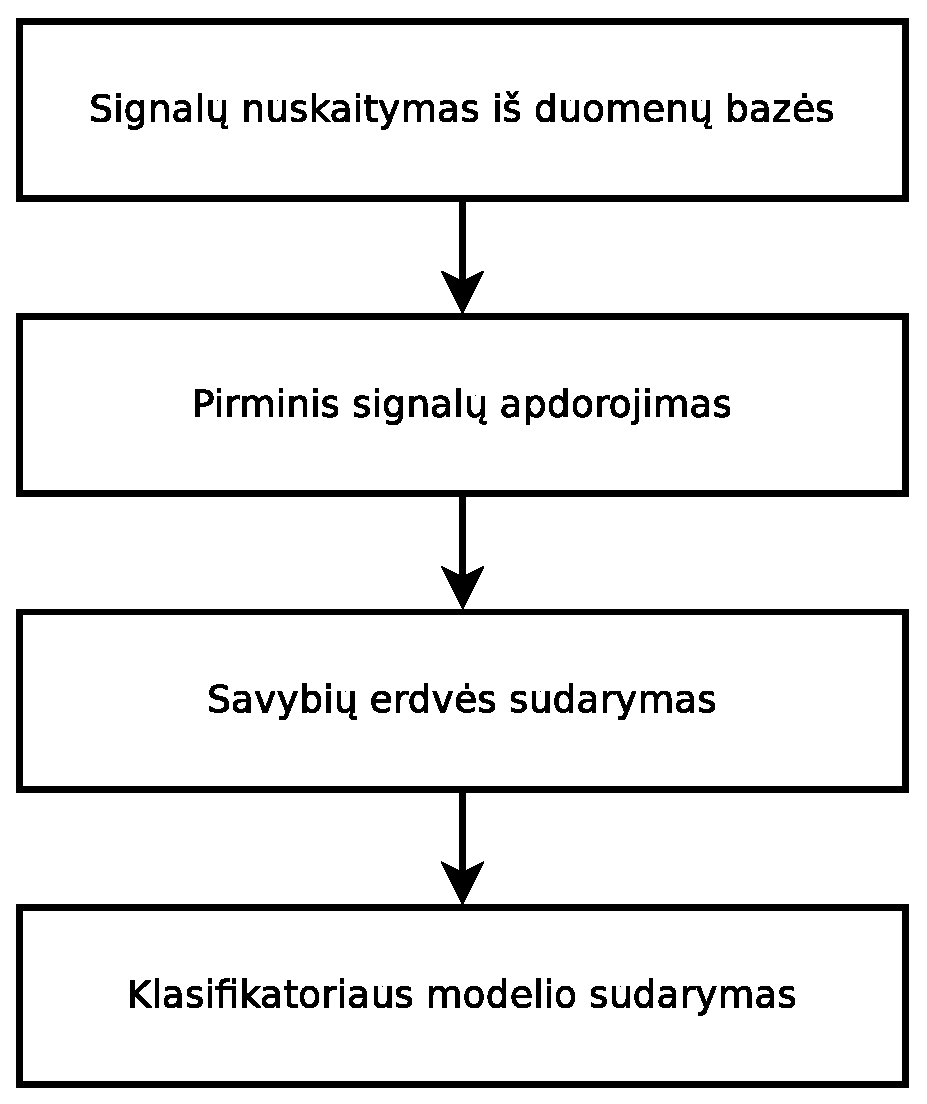
\includegraphics[width=200px]{figures/pirmine_schema.eps}
  \caption{Pirminė programos schema.}
  \label{fig:pirmine_programos_schema}
\end{figure}

Priklausomai nuo taikomos metodikos, programos struktūrinės schemos skiriasi, kadangi vienas sprendimas reikalauja vieno tipo duomenų struktūros, kitas - kitos struktūros. Programos projektavimo metu buvo išbandyti keli programos variantai ir suprastinus veikimo schemas, kiekvienas iš programos variantų veikė pagal bendrą schemą, kurią galima apibrėžti \ref{fig:pirmine_programos_schema} pav. Reikalaujama, kad kiekvienas iš algoritmų blokų būtų nepriklausomas nuo žemiau ar aukščiau einančio bloko, kas reiškia, kad ``Pirminio signalų apdorojimo'' bloko algoritmo pakeitimas neturi turėti jokios įtakos po jo einančiam ``Savybių erdvės sudarymas'' blokui. 

Kiekvieno bloko užduotis:

\begin{enumerate}
\item ``Duomenys iš duomenų bazės'' bloko užduotis yra nuskaityti iš naudojamos ``PhysioBank'' duomenų bazės duomenis ir juos įkrauti į Matlab aplinką. Kadangi duomenys pateikiami tekstiniu pavidalu, Matlab aplinkoje yra labai patogi funkcija tokiems duomenims nuskaityti - $dlmread$.

\item ``Pirminis signalų apdorojimas'' bloko užduotis yra pradinis signalų filtravimas, nuolatinės komponentės pašalinimas. Taip pat, į šį bloką įeina ir atskirų signalų išskyrimas iš bendrai gaunamo signalo: signalo išskyrimas kuomet koja turi susilietimą su žeme, signalo išskyrimas, kuomet koja praranda susilietimą su žeme. Į bloką taip pat įeina ir slankiojančio lango algoritmo taikymas.
\item ``Savybių erdvės sudarymas'' bloko paskirtis yra pateikti pasirinktam klasifikatoriui išskirtas signalų savybes po pirminio signalo apdorojimo. Tokiomis savybės gali būti signalų dažninės komponentės (Furjė koeficientai), koreliacijos koeficientai tarp dešinės ir kairės kojos, savi-koreliacijos koeficientai dešinės ar kairės kojos. Detaliau nagrinėjamas savybes bus aptartos tolimesniuose poskyriuose. Į bloką taip pat įeina ir darbas su dimensijomis - dimensijų skaičiaus mažinimas ar naujos erdvės paieška, kurioje nagrinėjami duomenys yra geriau tiesiškai atskiriami.

\item ``Klasifikatoriaus projektavimas'' bloko paskirtis yra klasifikatoriaus apmokymas ir jo testavimas. Klasifikatoriaus pasirinkimas yra labai svarbus klausimas nagrinėjamam darbe. Jis turi būti parinktas argumentuotai, pateikiant detalius klasifikavimo rezultatus, remiantis rezultato grafiku. Nepasitikėjimo matrica, bei iš jos apskaičiuotais įverčiais: taiklumu bei tikslumu. Dar svarbus klasifikatoriaus aspektas yra savybių erdvės bendro dėsnio radimas arba jo aproksimacija. Šį faktą galima apibrėžti iš klasifikavimo grafiko. Jeigu klasifikavimo rezultatas yra nestabilus, ilgą laiką neturintis pastovaus rezultato, vadinasi, galima teigti, kad klasifikatorius blogai atliko erdvės dėsnio aproksimavimą, jis nėra tinkamas nagrinėjamai savybių erdvei.
\end{enumerate}

Tolimesniuose poskyriuose bus aptarti įgyvendinti blokinės struktūros elementai.

\subsection{Pirminio signalų apdorojimo programos kūrimas}

Šiame skyriuje bus aptartas pirminio signalų apdorojimo programos kūrimas. Aptartas duomenų nuskaitymas iš duomenų bazės bylos tekstiniame pavidale, galimas signalo išskaidymas slankiojančio lango metodu arba signalo formos nuskaitymas, priklausomai nuo žinomo fizinio poveikio, kuriuo metu signalas buvo gautas.

Programos kūrimo patogumui, buvo parinkta direktorijų architektūra:

\begin{itemize}
\item Tėvinė direktorija
  \begin{itemize}
  \item <programos versija, nurodyta datos formatu>
  \item database
  \item cache
  \end{itemize}
\end{itemize}

Kadangi programos kūrimo metu yra svarbu saugoti ankstesnes programos versijas, buvo parinktas kasdienis programos versijos saugojimas: kiekvienos pradžioje darbas buvo pradedamas su ankstesnės dienos kopija. Taip buvo išsaugotas kiekvienos darbo dienos programos versija ir taip galima peržiūrėti kokiu analitiniu keliu buvo eita prie dabartinės programos versijos.

Pirmoji funkcija, priklausanti pirminio signalo apdorojimo programai yra $read\_data$. Funkcijos kodas pateikiamas \ref{code:read_data} pav.

\begin{cfigure}
  \centering
  \caption{Duomenų nuskaitymo funkcija iš tekstinės duomenų bylos.}
  \label{code:read_data}
  \lstinputlisting{sources/read_data.m}
\end{cfigure}

Funkcijai užtenka nurodyti tik norimos nuskaityti bylos pavadinimą, kaip pavyzdžiui ``SiPt30\_01.txt'' ir funkcija gražins kairės kojos duomenis. Duomenų analizėje naudojami tik vienos kojos duomenis, kadangi dešinės ir kairės kojos duomenys yra stipriai koreliuoti \cite{16053531}, todėl nėra prasmės naudoti dviejų kojų duomenų. Pasirinkus tokį sprendimą taip pat yra sumažinamas skaičiavimų skaičius programoje. Duomenų bazės direktorija nurodyti kintamojo vietoje yra taip pat svarbus aspektas, kadangi pakitus duomenų bazės vietai, užteks tik pakeisti vieną kintamąjį, o ne visą kodą, nors kodas ir nėra ilgas. Matlab funkcija $dlmread$ gražina duomenis masyvo pavidalu, kur stulpelis nurodo įvade aptartus duomenis, o eilutė nurodo duomenų vertes tam tikru laiko momentu.

\begin{cfigure}
  \centering
  \caption{Slankiojančio lango algoritmo pritaikymas.}
  \label{code:sliding_window}
  \lstinputlisting{sources/split_data.m}
\end{cfigure}

Sekantis žingsni, po duomenų nuskaitymo, yra jų pirminis apdorojimas. Nagrinėjimas bus pradėtas nuo slankiojančio lango metodo. Programos kodas pateikiamas \ref{code:sliding_window} pav. Funkcijos įvestyje pateikiamas nagrinėjamas signalas, slankiojamo lango ilgis ir slankiojamo lango perdanga. Slankiojamo lango perdanga nurodo reikšmių arba laiko verčių kiekį, kurį algoritmas pašalina iš spartinančiosios atminties, laukdamas naujų verčių langui užpildyti. Pavyzdžiui, jeigu lango ilgis yra 4 signalo verčių, o perdanga - 2 signalo vertės, vadinasi, kai algoritmas užpildys langą 4 signalo vertėm, esamą langą jis perduos į išėjimo spartinančiąją atmintį, paskutines dvi vertes ištrins iš spartinančiosios atminties ir iš naujo lauks naujų dviejų reikšmių langui pilnai užpildyti.

Funkcija yra tiek lanksti, kad nėra svarbu kokio tipo duomenys yra pateikiami - ar tai konkretaus signalo vertės ar iš ankščiau pritaikyto slankiojančio lango algoritmo išskirtos signalo savybės, kuriuos buvo panaudotos formuojant naują signalą. Tokia funkcijos savybė bus labai naudinga tolimesniame darbe.

\begin{cfigure}
  \centering
  \caption{Signalo filtravimas dviem Butterworth filtrais.}
  \label{code:filter}
  \begin{lstlisting}
    [B,A] = butter(9, 1/50, 'high');
    [BB,AA] = butter(9, 40/50, 'low');
    output = filter(BB, AA, filter(B, A, input));
  \end{lstlisting}
\end{cfigure}

Sekanti programos dalis atlieka paprastą signalo filtravimą su dvejais $Butterworth$ skaitmeniniais filtrais. Pirmasis, aukštų dažnių filtras, skirtas pašalinti signalo nuolatinei komponentei. Antras, žemų dažnių filtras, skirtas pašalinti aukšto dažnio triukšmą, kuris neneša visiškai jokios naudingos informacijos. Filtras įgyvendinamas labai paprastai. Kodo pavyzdys pateikiamas \ref{code:filter} pav. Abiejų filtrų eilė yra 9-ta, žemų dažnių filtro ribinis dažnis parinktas $40~Hz$. Duomenys diskretizuojami $100~Hz$ dažniu, vadinasi didžiausias galimas signalo dažnis yra $50~Hz$. Didžiausias žmogaus generuojamas dažnis ėjimo metu, remiantis šaltiniu, yra $20~Hz$. Užtikrintumui buvo parinktas $40~Hz$ dažnis. Nuolatinė dedamoji pašalinama su aukšto dažnio filtru, kurio ribinis dažnis yra $1~Hz$. Nuolatinė dedamoji neneša jokios informacijos apie eisena, kadangi ji tiktais nurodo naudojamų jutiklių jautrumą.

\begin{cfigure}
  \centering
  \caption{Kontakto su žeme signalo išskyrimo programos kodo fragmentas.}
  \label{code:signal_extraction}
  \lstinputlisting{sources/extract_signal.m}
\end{cfigure}

Toliau seka, priklausomai nuo pasirinkto pirminio signalų apdorojimo būdo, signalo išskyrimas pagal fizinę veiklą. Dominančios signalo būsenos yra, kai subjekto koja turi kontaktą su žeme ir nurodytas subjektas neturi kontakto su žeme. Kontakto su žeme signalo išskyrimui programos kodas yra pateikiamas \ref{code:signal_extraction} pav.

Pirmiausiai, ``Pt\_t'' kintamojo struktūroje yra saugoma kairės kojos Parkinsono liga sergančių subjektų duomenys. Kiekvienas signalas yra priskiriamas prie $signal$ kintamojo, su kuriuo toliau yra tęsiamas apdorojimo procesas. Jeigu signalas nėra lygus nuliui, tuomet jis įdedamas į laikinąją atmintį. Taip signalas yra tikrinamas iki tol, kol signalas tampa lygus nuliui ir tęsiamas tolimesnis apdorojimas. Apdorojimas susideda iš signalo ilgio patikros. Jeigu signalas yra trumpesnis už 10 verčių, arba turint omenyje, kad signalas buvo diskretizuojamas $100~Hz$, tai $0.1~s$, vadinasi, signalas yra tiesiog aukšto dažnio triukšmas arba blogas pavyzdys ir signalas yra atmetamas. Jeigu signalas yra ilgesnis už 200 verčių ($2~s$), vadinasi, duomenų rinkimo metu įvyko klaida ir koja per tokį laiką pakelta nebuvo. Tokia klaida gali būti sukelta, kuomet subjektas ne eina, o stovi ant dviejų kojų arba tik ant kairės kojos. Jeigu visi kriterijai patenkinami, signalas yra priimamas ir kraunamas į laikinąją atmintį, pavadinimu ``$data.Pt$''. Signalas, kuriuo metu koja neliečia žemės, yra randamas kartu su ankščiau išnagrinėtu metu. Algoritmas patikrina kiek praėjo laiko (arba kiek verčių yra priskaičiuota) nuo paskutinio užskaityto kojos ant žemės signalo ir įrašo tą signalą į laikiną atmintį, jeigu po praeito signalo nepraėjo mažiau negu 50 verčių arba $0.5~s$ ir nedaugiau nei 200 verčių arba $2~s$. Kojos signalas yra pateiktas \ref{fig:stance_phase} pav.

\begin{figure}[!t]
  \centering
  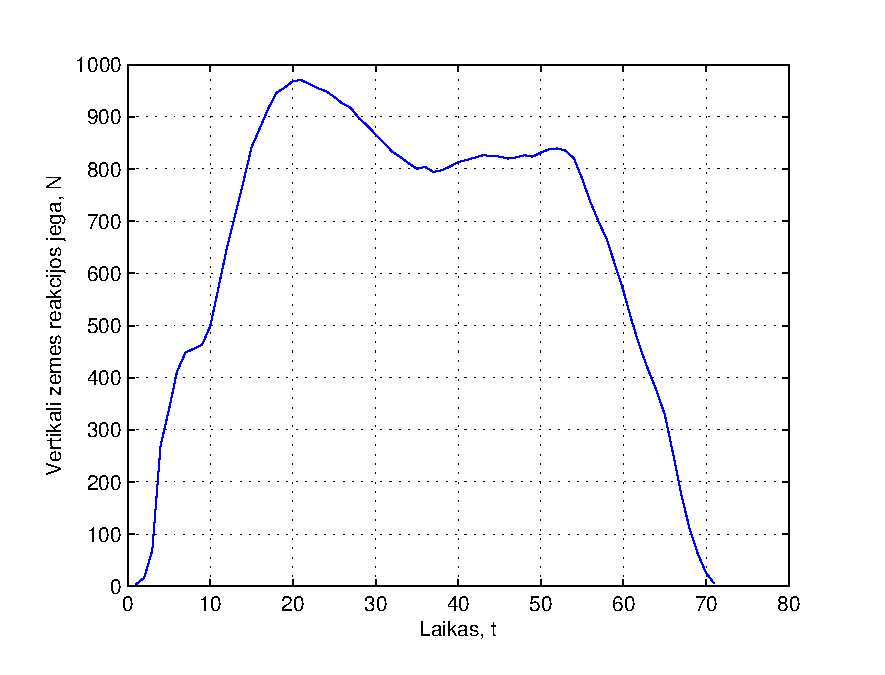
\includegraphics[width=300px]{figures/09_sample_stance_phase.eps}
  \caption{Susilietimo su žeme signalas.}
  \label{fig:stance_phase}
\end{figure}

\begin{figure}[!t]
  \centering
 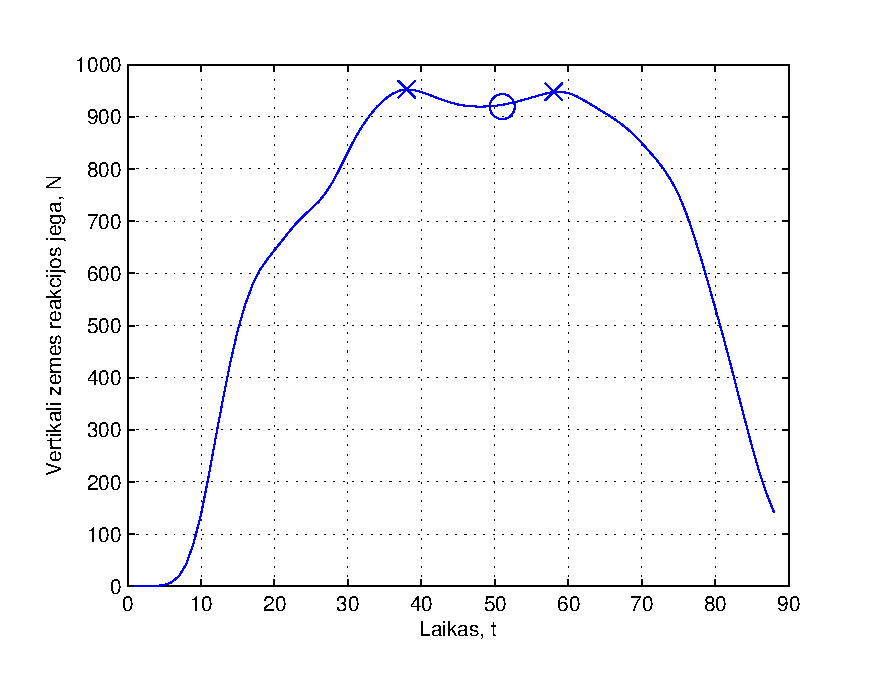
\includegraphics[width=300px]{figures/10_global_max_local_min.eps}
  \caption{Dviejų globalių maksimumų ir vieno lokalaus minimumo
    radimas signale.}
  \label{fig:min_max}
\end{figure}


% TODO: ref

Dar vienas pirminis signalo apdorojimas, kurį teko panaudoti tiriant galima bendrą erdvę - kiekvieno kojos susilietimo su žeme signalo dviejų globalių maksimumų ir vieno lokalaus minimumo paieška \cite{6151536}. Algoritmo rezultatas yra pateiktas \ref{fig:min_max} pav. Kryžiais pažymėtos globalaus maksimumo vietos, apskritimu pažymėta lokalaus minimumo signalo vieta. Išanalizavus daugumos subjektų žingsnio signalus, buvo padaryta išvada, kad kiekviename žmogaus žingsnyje egzistuoja du maksimumai. Vienas maksimumas randamas, kai subjektas yra visiškai atsirėmęs galine pėdos dalimi į žemę, antras maksimumas randamas, kai subjektas visiškai atsiremia priekinę pėdos dalimi. Tarp šių dviejų maksimumų yra pereinamasis laikotarpis, kuris yra signalo lokalus minimumas. Priežastis, dėl kurios algoritmas buvo įgyvendintas, yra vienas darbas, kuriame buvo pasiūlyta naudotis būtent tokiomis savybėmis atpažinti Parkinsono liga sergančius subjektus nuo nesergančių subjektų. Pačio algoritmo kodo dalis yra pateikta \ref{code:min_max} pav.

\begin{cfigure}[!t]
  \centering
  \caption{Dviejų globalių maksimumų ir vieno lokalaus minimumo radimo algoritmo fragmentas.}
  \label{code:min_max}
  \lstinputlisting{sources/min_max.m}
\end{cfigure}

Programos kodas krauna gaunamą signalą į laikinąją atmintį ir tikrina ar signalas pakito per užduotą dydį $\delta$. Delta nurodo kiek signalas turi pakisti, kad algoritmas nuspręstų, kad signalas pradėjo mažėti. Tokio tikrinimo priežastis yra ta, kad prieš globalų maksimumą taip pat yra sritis, kurioje signalas kilimas sulėtėja, o kai kuriuose pavyzdžiuose buvo pastebėta, kad signalas net pradeda mažėti. Dėl šios priežasties buvo įvesta pokyčio tikrinimo sąlygą.

Pirminio signalų apdorojimo programa baigiasi nurodytais metodais. Sekantis žingsnis yra apdorotų duomenų perdavimas tolimesnei programos pakopai - požymių išskyrimui.

\subsection{Požymių išskyrimo programos kūrimas}

Požymių išskyrimas priklauso nuo pirminio signalo apdorojimo mechanizmo. Jeigu ankstesniame bloke pakeisime ribinį filtro dažnį ir kaip nagrinėjamą požymį bus parinktas koreliacijos koeficientai ar dažninės komponentės - požymio vektorius pakis, todėl prieš kiekvieną požymių analizavimo ciklą bus pateikta ir pirminiam signalų apdorojimo bloke naudojami metodai. Taip pat, kadangi požymių išskyrimo programos kūrimas taip pat sprendžia ir dimensijų klausimą - skyriaus pradžioje bus trumpai apžvelgti populiariausi šiame darbe panaudoti dimensijų mažinimo metodai.

\subsubsection{Dimensijų mažinimas}

Dimensijų mažinimas suteikia dideles galimybes supaprastinti klasifikavimo uždavinį. Kuomet duomenys savybių erdvėje nėra linijiškai atskirti, yra sunku nustatyti ar klasifikatorius ras apibendrintą duomenų praskyrimo funkciją. Norint užtikrinti, kad klasifikatorius veiks teisingai - yra atliekamas dimensijų praskyrimas. Metodas taip pat taikomas, kuomet norima sumažinti dimensijų skaičių. Problema iškyla, kuomet norima įgyvendinti sukurtą sprendimą įterptinėje sistemoje, kurioje negalima pasiekti didelių aparatinių resursų. Turint didelių dimensijų duomenis taip pat kyla ir pačios sistemos kaina, dėl tų pačių aparatinių resursų reikalavimų. Norint išvengti tokių problemų - taikomi dimensijų mažinimo algoritmai. Populiariausi dimensijų mažinimo algoritmai yra:

\begin{itemize}
\item Linijinė diskrtiminanto analizė (angl. Linear Discriminant Analysis (LDA));
\item Principinė komponenčių analizė (angl. Principal Component Analysis (PCA)).
\end{itemize}

Taip pat, kiekvienas iš paminėtų būdu taip pat gali būti papildytas branduolio (angl. Kernel) funkcija. Metodų apibūdinimas bus pradėtas nuo paprasčiausios iš dviejų - PCA.

Principinė komponenčių analizė \cite{citeulike:2695782} yra statmena ir paprasta transformacija, kuri yra daug kur naudojama dėl paprastos matematinės pusės ir lengvo įgyvendinimo. Egzistuoja skirtingi PCA metodo įgyvendinimo algoritmai. Vienas iš jų yra vienetinės reikšmės skaidymas (angl. Singular Value Decomposition (SVD)). Literatūroje PCA ir SVD dažniausiai minimi kaip sinonimai. SVD yra greitas, tačiau didelių atminties resursų reikalaujantis metodas. Kuomet dideli atminties resursai nėra prieinami (įterptinėje sistemoje), reikia naudoti kitą įgyvendinimo variantą - naudoti tikrinių vektorių skaidymą. Toks sprendimas užima didesnius laiko resursus, lyginant su SVD, tačiau jam reikia mažesnių atminties resursų ir jis tinka nagrinėti didelių dimensijų duomenis. Toks sprendimas bus taikomas ir šiame darbe. PCA įgyvendinimas naudojant SVD ir tikrinių vektorių skaidymą yra pateiktas priede. Toliau bus išnagrinėtas PCA iš matematinės pusės.

Matematiškai, PCA apibrėžiamas kaip statmena linijinė transformacija, kuri transformuoja duomenis į naują koordinačių sistemą, kurioje didžiausią variaciją projektuojama į pirmą ašį, antroji didžiausia variacija (statmena pirmajai) projektuojama į antrą ašį. Procesas tęsiasi tol, kol yra pasiekiamas norimas dimensijų skaičius.

Apibrėžta duomenų matrica $\textbf{X}^T$, su empiriniu vidurkiu, kuris lygus nuliui (empirinis vidurkis reiškia vidurkio apskaičiavimą ir jo atėmimą iš duomenų), kur kiekviena eilutė $n$ atspindi duomenų rinkinį, o stulpelis $m$ - turimas duomenų dimensijas. Matricos $\textbf{X}$ vienetinės reikšmės skaidymas išreiškiamas:

\begin{equation}
  \mathbf{X} = \mathbf{W} \Sigma \mathbf{V}^T,
\end{equation}
kur $m*n$ matrica $\mathbf{W}$ yra matricos $\textbf{XX}^T$ tikrinių vektorių matrica, $\Sigma$ matrica yra $m*n$ stačiakampio įstrižainės matrica su realiais skaičiais įstrižainėje ir $n*n$ tikrinių vektorių $\mathbf{X}^T\mathbf{X}$ matrica $\mathbf{V}$. PCA transformacija, kuri sukonstruoja naujas dimensijas, yra apibrėžiama:

\begin{equation}
  \mathbf{Y}^T = \mathbf{X}^T \mathbf{W} = \mathbf{V} \Sigma^T
  \mathbf{W}^T \mathbf{W} = \mathbf{V} \Sigma^T .
\end{equation}

Kadangi $\textbf{W}$ yra statmena matrica, kiekviena $\textbf{Y}^T$ eilutė yra matricos $\textbf{X}^T$ eilutės sukimas. Pirmasis $\textbf{Y}^T$ stulpelis yra pirmosios komponentės rezultatas, antras stulpelis yra antrosios komponentės rezultatas. Kiek stulpelių $\textbf{Y}^T$ turi, tiek ir rezultatų (dimensijų) yra po transformacijos.

Linijinė diskriminanto analizė \cite{welling2005fisher} yra dimensijų mažinimo metodas (kuris kartu yra naudojamas kaip ir klasifikatorius), yra vienas iš metodų, kuris neša kartu ir duomenų žymėjimo informaciją. Tai reiškia, kad mažinant dimensijų skaičių, metodas turi žinoti kokie duomenys priklauso kokiai duomenų klasei. Pagrindinis LDA tikslas yra didinti sekantį kriterijų:

\begin{equation}
  \mathfrak{J}(\mathbf{w}) = \frac{ \mathbf{w}^T S_B \mathbf{w} }{
    \mathbf{w}^T S_W \mathbf{w} },
\end{equation}
kur $S_B$ yra ``išorinės klasės scatter matrica'', $S_W$ yra ``vidinė klasės scatter matrica''. Scatter matricų apibrėžimas yra:

\begin{equation}
  S_B = \sum_c (\mu_c - \bar{x})(\mu_c - \bar{x})^T
\end{equation}

\begin{equation}
  S_W = \sum_c \sum_{i \in c} ( x_i - \mu_c)(x_i - \mu_c)^T
\end{equation}

%% Branduolio metodas

Branduolio metodas yra labai lengvai paaiškinamas pavyzdžiu \cite{2007math......1907H}. Tarkim, egzistuoja tam tikri empiriniai duomenys:

\begin{equation}
  (x_1,y_1),...,(x_n,y_n) \in \mathcal{X} \times \mathcal{Y}.
\end{equation}

Čia, $\mathcal{X}$ yra netuščia sritis, iš kurios imami $x_i$ duomenys. Tikslu arba žymekliu vadinami yra $y_i \in \mathcal{Y}$ (sistemos atsakas), $i,j \in [n]$ žymimas eilės, identifikavimo numeris, kur $n := \{1,..,n\}$.

Reikia pastebėti, kad sričiai $\mathcal{X}$ nebuvo suteikta jokių apribojimų. Norint išspręsti apmokymo problemą reikia papildomos struktūros. Mašininiame apmokyme siekiama apibendrinti neturimus duomenis. Binarinio klasifikavimo atveju, turint naujus duomenis $x \in \mathcal{X}$, norima nuspėti jų žymeklį $y \in \{\pm 1\}$. Paprastai kalbant, norima pasirinkti tokį $y$, kuris labiausiai atspindėtų apmokymo metu naudotas $(x,y)$ poras. Tam įgyvendinti reikalingi kuo panašesnis duomenys į $\mathcal{X}$ ir $\mathcal{Y}$. Pastarąjį palengvina tai, kad spėjimas gali būti arba identiškas arba atvirkščias. Formaliai yra reikalinga tokia funkcija:

\begin{equation}
  k: \mathcal{X} \times \mathcal{X} \rightarrow \mathbb{R}, ~~ (x,x')
  \rightarrow k(x,x'),
\end{equation}
kuri tenkinta tokias sąlygą visiems $x,x' \in \mathcal{X}$:

\begin{equation}
  k(x,x') = \langle \Phi(x), \Phi(x') \rangle,
\end{equation}
kur $\Phi$ projektuota taškus į Hilberto plokštumą $\mathcal{H}$, kai kada vadinama savybių erdvė. Vienodumo matmuo $k$ dažniausiai vadinamas branduoliu, o $\Phi$ vadinama savybių projekcija.

\subsubsection{Savybių tyrimas}

Šiame skyriuje bus išnagrinėtos galimos signalų savybės, pagal kurias galima atskirti Parkinsono liga sergantį subjektą nuo sveiko subjekto. Kaip buvo minėta ankščiau, ne visos savybės gali būti išskirtos, naudojantis vienu pirminio signalo apdorojimo mechanizmu, todėl kiekvienos savybės nagrinėjimo pradžioje bus paminėta ir pirminio signalo apdorojimo bloko sudėtis.

% TODO: reference

Galimų savybių analizavimas gali būti pradėtas nuo signalo dažninių komponenčių (Furjė transformacijos). Kaip nurodo šaltiniai,  Parkinsono liga sergančių subjektų žingsniai turi statesnius šlaitus, kas iš signalų apdorojimo srities reiškia, kad signalas turi turėti aukštas dažnines komponentes. Šiai savybei išskirti pirminiam signalo apdorojimo bloke bus panaudotas slankiojančio lango metodas. Taip kiekvienas signalas turės fiksuotą ilgį ir taip bus galima lyginti signalus tarpusavyje.

\begin{figure}[!t]
  \centering
  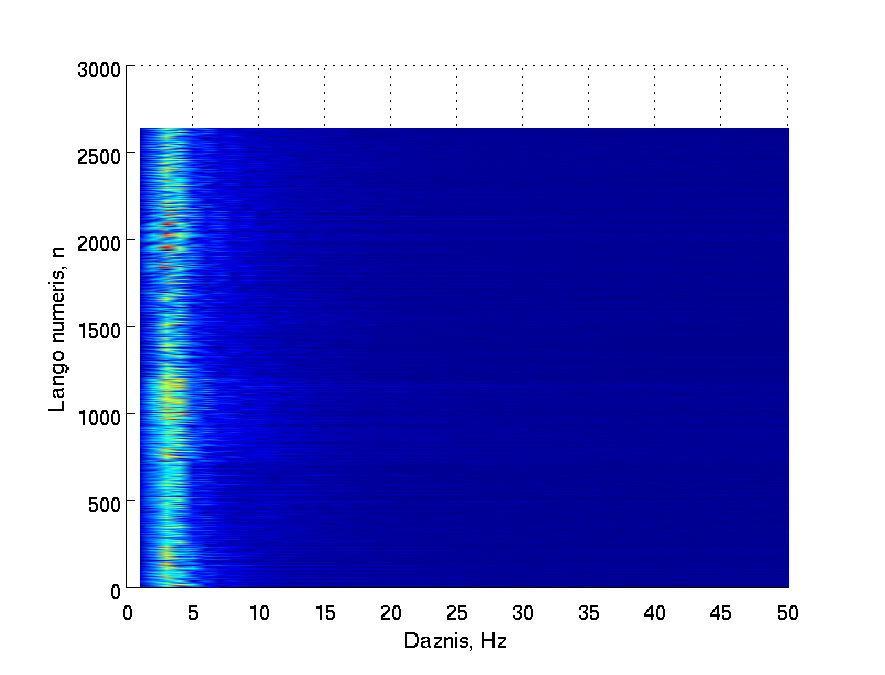
\includegraphics[width=300px]{figures/co_fft.eps}
  \caption{Kontrolinių subjektų kairės kojos žingsnių signalų dažninės
  komponentės}
  \label{fig:co_fft}
\end{figure}

\begin{figure}[!t]
  \centering
  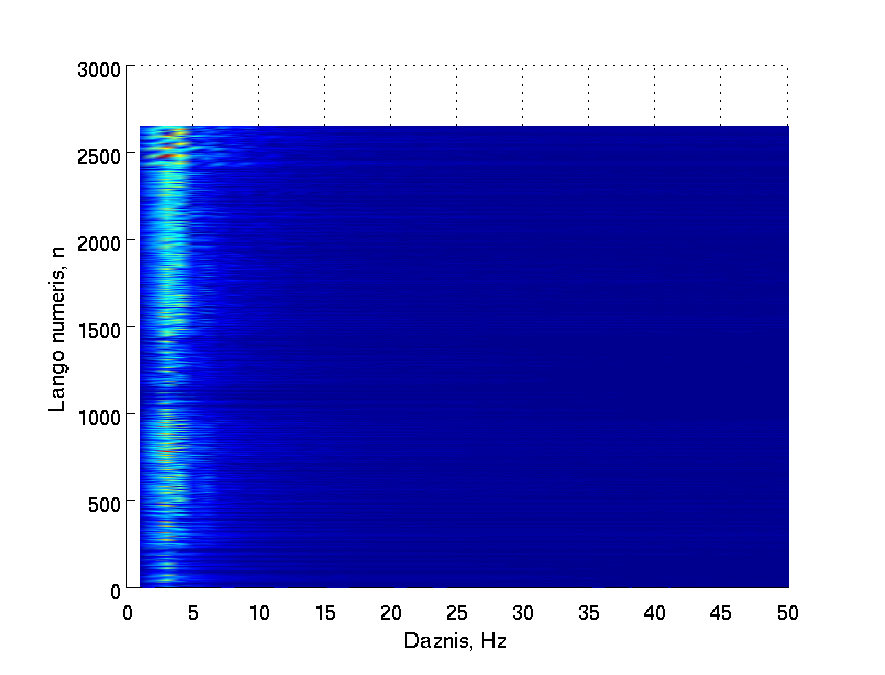
\includegraphics[width=300px]{figures/pt_fft.eps}
  \caption{Parkinsono liga sergančių subjektų kairės kojos žingsnių signalų dažninės
  komponentės}
  \label{fig:pt_fft}
\end{figure}


Toliau bus išanalizuoti Parkinsono liga sergančių subjektų ir kontrolinių subjektų žingsnių signalų dažninės komponentės. Kontrolinių subjektų kairės kojos žingsnių dažninės komponentės yra pateiktos \ref{fig:co_fft} pav. Parkinsono liga sergančių subjektų kairės kojos žingsnių dažninės komponentės yra pateiktos \ref{fig:pt_fft} pav. Kaip matoma iš duotų komponenčių grafikų - tiek kontrolinių subjektų, tiek Parkinsono liga sergančių subjektų pagrindinės dažninės komponentės išsidėsto iki $5~Hz$ ruože. Ties $0~Hz$ dažninių komponenčių nėra, kadangi jos buvo pašalintos filtro pagalba. Už $10~Hz$ ribos, komponentės neneša visiškai jokios informacijos. Iš to galima padaryti išvadą, kad tiek Parkinsono liga sergančių subjektų, tiek kontrolinių subjektų eisenos yra visiškai vienodos dažnių srityje ir vien remiantis šita informacija nėra galima nustatyti ar subjektas serga Parkinsono liga ar ne.

Tolimesnė analizė gali būti atlikta, remiantis koreliacijos koeficientais. Analizuojant šias savybes, galima remtis tokiu pačiu pirminiu signalo apdorojimo bloku, kaip ir analizuojant dažnines komponentes. Dėl to, kad esama tikrais kairės kojos sinalai, alima taikyti tik savi-koreliacijos koeficientus. Narinėjama savybė parodė labai gerus rezultatus ankstesniame tyrime, kuriame, remiantis akselerometro ir giroskopo jutiklių parodymais, reikėjo suprojektuoti algoritmą, gebantį atskirti tokias žmogaus veiklas: stovėjimas, ėjimas, ėjimas aukštyn laiptais, ėjimas žemyn laiptais.

\begin{figure}[!t]
  \centering
  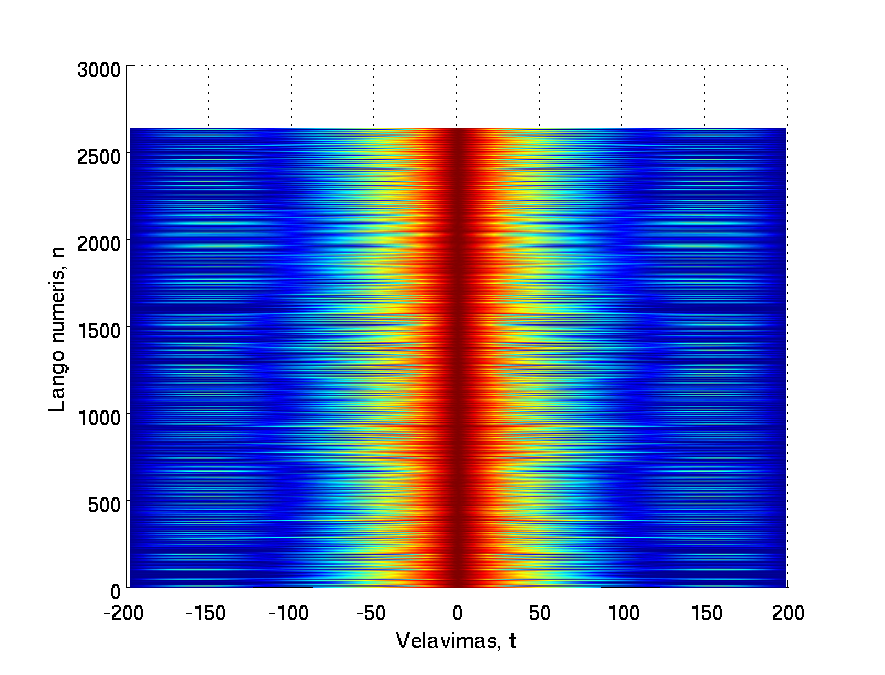
\includegraphics[width=300px]{figures/co_corr.eps}
  \caption{Kontrolinių subjektų kairės kojos žingsnių signalų
    savi-koreliacijos koeficientai.}
  \label{fig:co_corr}
\end{figure}

\begin{figure}[!t]
  \centering
  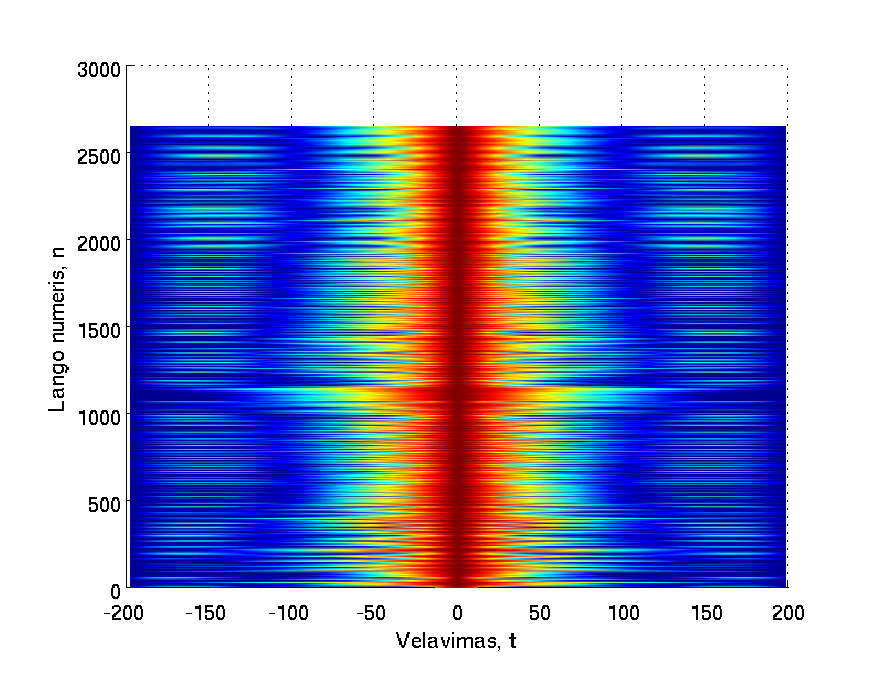
\includegraphics[width=300px]{figures/pt_corr.eps}
  \caption{Parkinsono liga sergančių subjektų kairės kojos žingsnių
    signalų savi-koreliacijos koeficientai.}
  \label{fig:pt_corr}
\end{figure}

Kontrolinių subjektų kairės kojos savi-koreliacijos koeficientai parodyti \ref{fig:co_corr} pav. Parkinsono liga sergančių subjektų kairės kojos savi-koreliacijos koeficientai parodyti \ref{fig:pt_corr} pav. Kaip matosi iš korelogramos, tiek sergantys, tiek kontroliniai subjektai turi panašias, o kai kuriais atvejais ir tokias pačias, koreliacijos reikšmes. Remiantis vien tik turima informacija, nustatyti ar subjektas serga Parkinsono liga ar ne, nėra įmanoma.

\begin{figure}[!t]
  \centering
  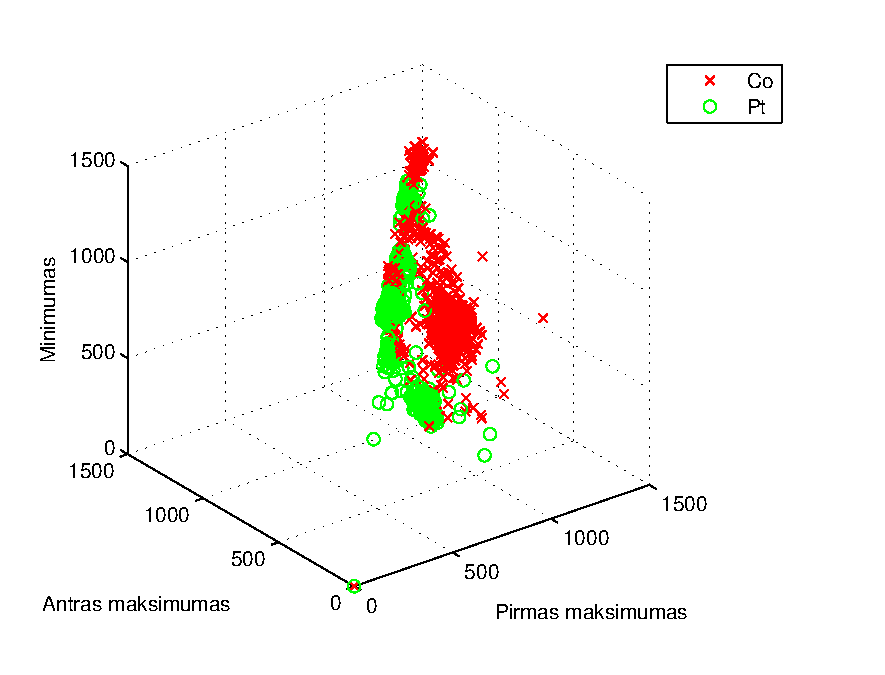
\includegraphics[width=300px]{figures/maximums_minimums.eps}
  \caption{Dviejų globalių maksimumų ir vieno lokalaus minimumo
    savybių erdvė.}
  \label{fig:max_min}
\end{figure}

Sudėtingesnė analizė seka iš dviejų globalių maksimumų ir vieno lokalaus minimumo savybių erdvės. Šios tris savybės sudaro trijų dimensijų plokštumą, kurią galima lengvai pavaizduoti. Pilna savybių erdvė pavaizduota \ref{fig:max_min} pav. Kaip matosi iš duotos erdvės, duomenys neturi jokio koncentracijos centro. Erdvėje jie pasiskirstę pagal nežinomą dėsnį.

Tokių duomenų pateikti klasifikavimui nėra galima. Grafike ``Co'' taškai, pažymėti kryžiumi, parodo kontrolinį subjektą, ``Pt'' taškai, pažymėti apskritimu, parodo Parkinsono liga sergančius subjektus.

Sekančios savybės nagrinėjimui yra siūlomos atliktų tyrimų \cite{16053531,KNUTSSON01011972,Delval_Salleron_Bourriez_Bleuse_Moreau_Krystkowiak_Defebvre_Devos_Duhamel_2008}. Nagrinėjama savybė yra žingsnio fazės laiko variacija. Kojos susilietimo su žeme laiko variacija ir kojos pakilimo nuo žemės laiko variacija.

\begin{figure}[!t]
  \centering
  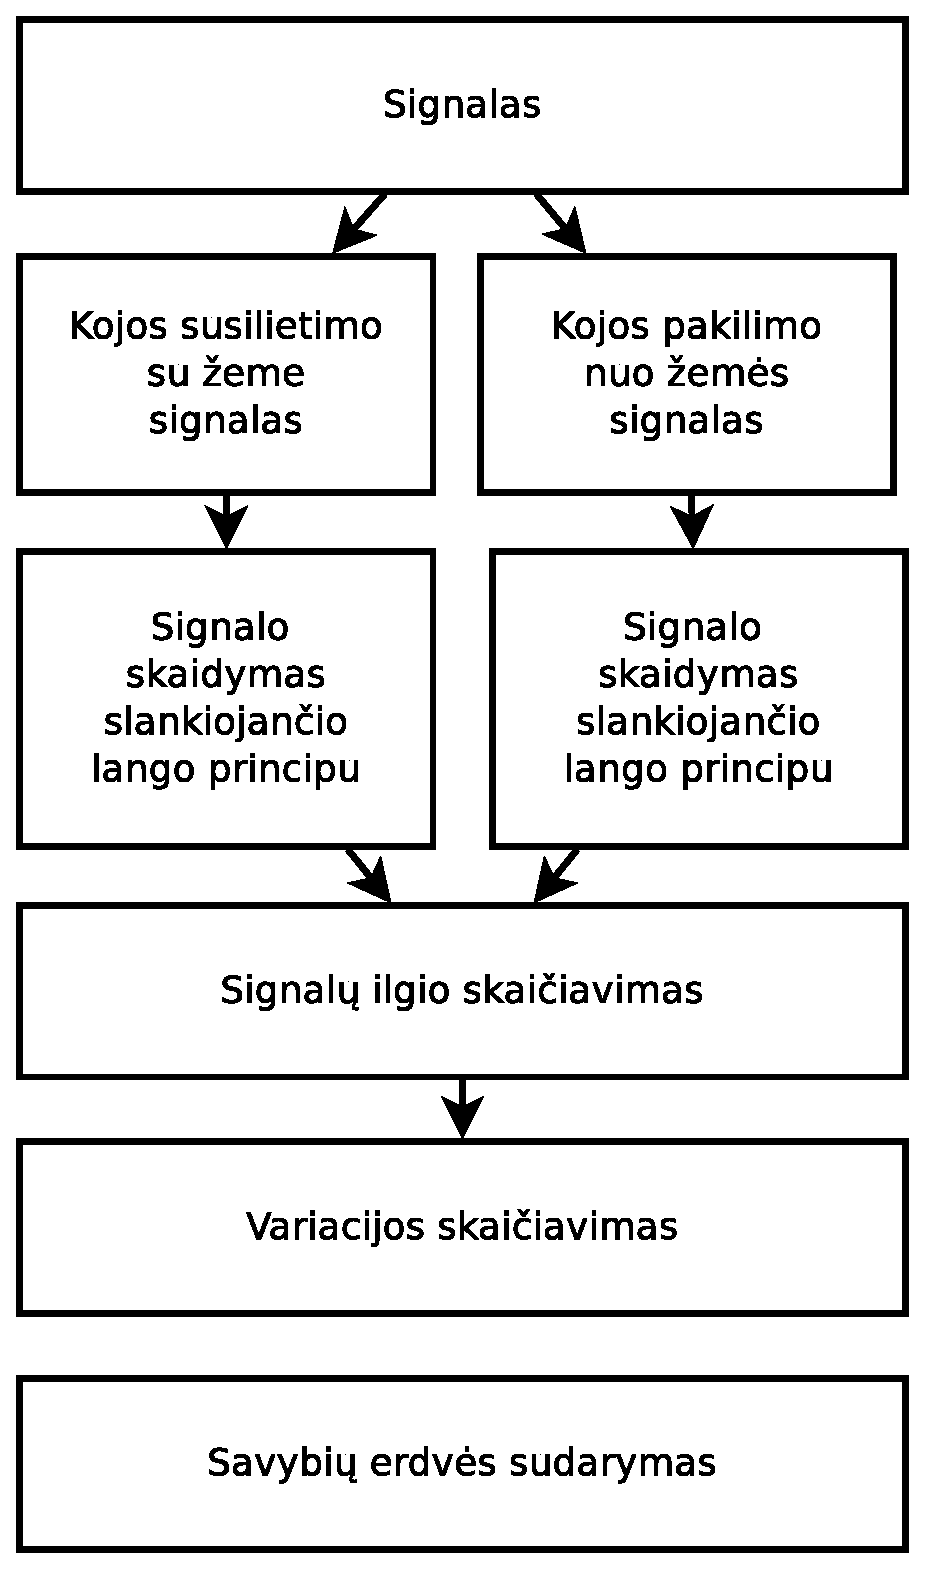
\includegraphics[width=200px]{figures/pirminis_signalo_apdorojimas_skaiciuojant_variacija.eps}
  \caption{Pirminis signalo apdorojimas, išskiriant savybę kaip kojos
    susilietimo su žeme laiko variaciją ir kojos pakilimo nuo žemės
    laiko variaciją.}
  \label{fig:stance_swing_extract}
\end{figure}

Išskiriant variacijos savybes iš signalo, reikalinga nuo pagrindų pakeisti pirminio signalo apdorojimo algoritmą. Kadangi kojos pakilimas nuo žemės ir kojos susilietimas su žeme gali būti vienas nuo kito nepriklausomi (subjektas sustojo ir stovi dviem kojomis ant žemės arba subjektas stovi tik ant kairės kojos), pirminis signalo apdorojimas turi būti atliekamas lygiagrečiai, t.y. tuo pat metu išskiriamas tiek kojos pakilimo nuo žemės signalas, tiek ir kojos susilietimas su žeme signalas. Tokios sistemos struktūrinis grafikas yra parodytas \ref{fig:stance_swing_extract} pav. Sekantis žingsnis yra signalo išskaidymas slankiojančio lango principu. Abiejų signalų slankiojančio lango ilgis buvo parinktas 4 verčių ilgio, su 2 verčių perdanga. Kuomet tiek kojos susilietimo su žeme, tiek kojos pakilimo nuo žemės keturi signalai patenkina keliamus reikalavimus - iš jų yra apskaičiuojami signalų ilgiai. Vėliau, abiejų etapų signalams yra paskaičiuojama jų variacija ir taip yra sudaroma savybių erdvė. Toliau bus nagrinėjamos abiejų signalų variacijos vienos dimensijos plokštumoje.

\begin{figure}[!t]
  \centering
  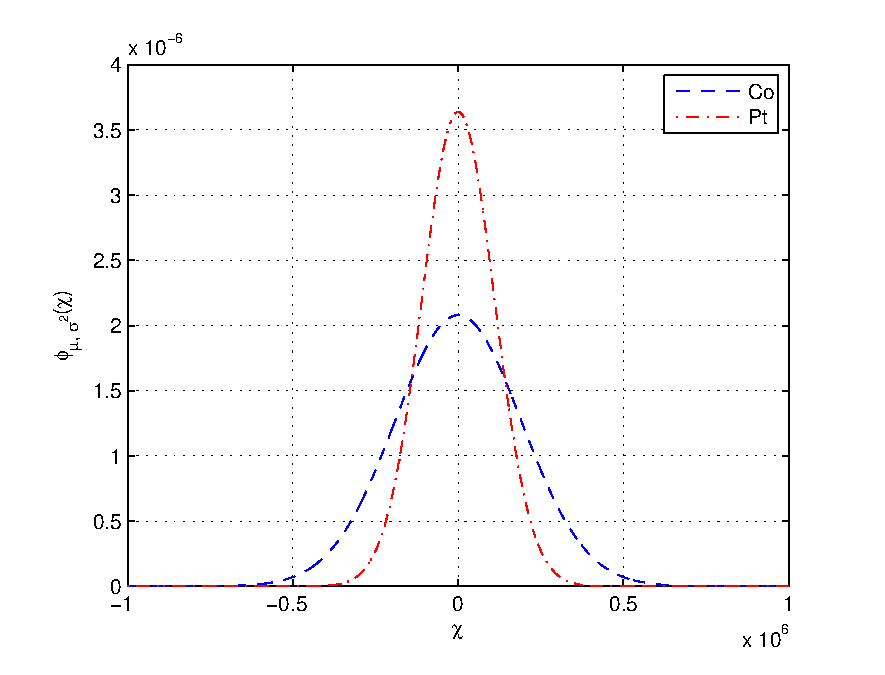
\includegraphics[width=250px]{figures/stance_phase.eps}
  \caption{Kojos prisilietimo prie žėmės laiko variacija.}
  \label{fig:stance_var}
\end{figure}

\begin{figure}[!t]
  \centering
  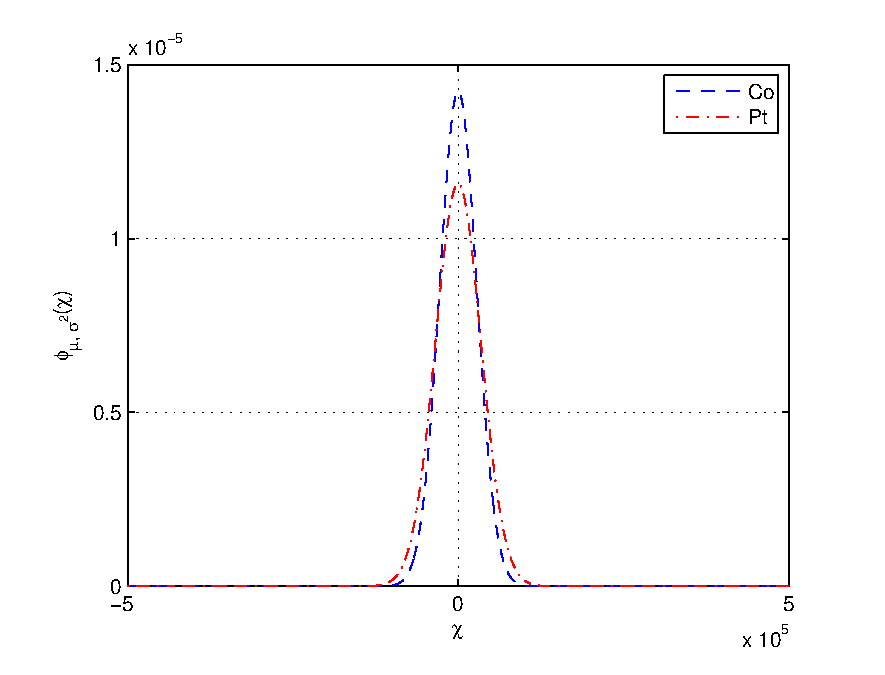
\includegraphics[width=250px]{figures/swing_phase.eps}
  \caption{Kojos pakilimo nuo žemės laiko variacija.}
  \label{fig:swing_var}
\end{figure}

Abiejų signalų variacijų pasiskirstymai yra parodyti \ref{fig:stance_var} pav. ir \ref{fig:swing_var} pav. Abu pasiskirstymai turi vieną trūkumą - jų vidurkiai sutampa, tačiau gera žinia yra tai, kad jų variacijos skirtingos. Norint išspręsti iškilusią problemą, reikia taikyti dimensijų praskyrimo metodus. Darbo metu buvo išbandyti tokie dimensijų praskyrimo metodai:

\begin{itemize}
\item PCA;
\item LDA;
\item Kernel PCA (su polinominiu, Gauso branduoliais);
\item Kernel LDA (su polinominiu, Gauso branduoliais);
\end{itemize}

\begin{figure}[!t]
  \centering
  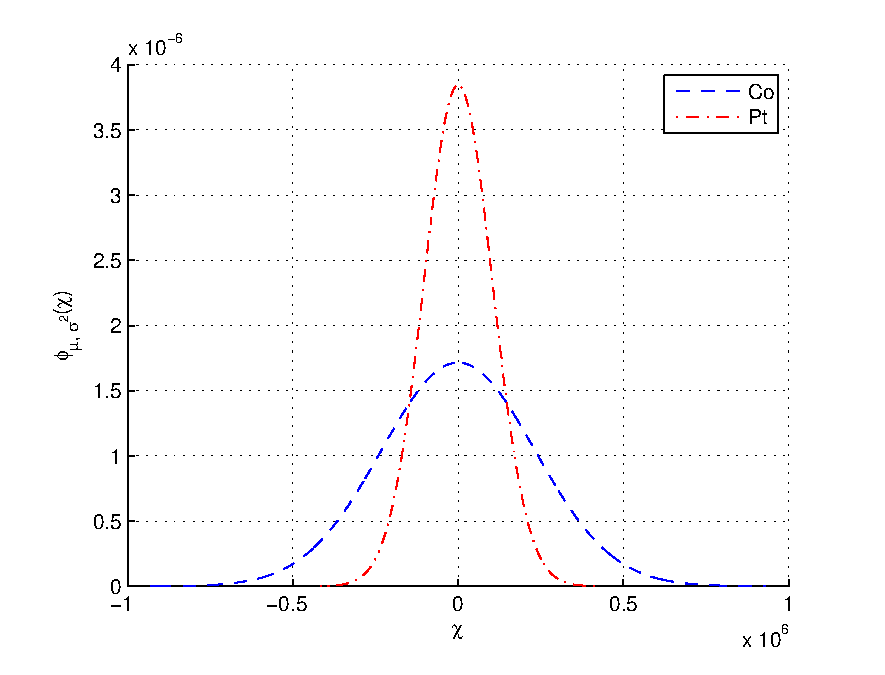
\includegraphics[width=250px]{figures/st_sw_linear_kpca.eps}
  \caption{Kojos prisilietimo prie žemės ir pakilimo nuo žemės laiko
    variacijos pasiskirstymas po PCA transformacijos.}
  \label{fig:linear_pca}
\end{figure}

Vienmatė linijinė PCA transformacija pavaizduota \ref{fig:linear_pca} pav. Kaip matosi iš grafiko - vidurkis nepasikeitė, tačiau žymiai pasikeitė variacija. Vidurkio pokyčio nebuvimas pablogina situacija, kadangi to pačio vidurkio duomenis atskirti nėra įmanoma, todėl ir teikti duomenis klasifikavimui nėra prasmės.

\begin{figure}[!t]
  \centering
  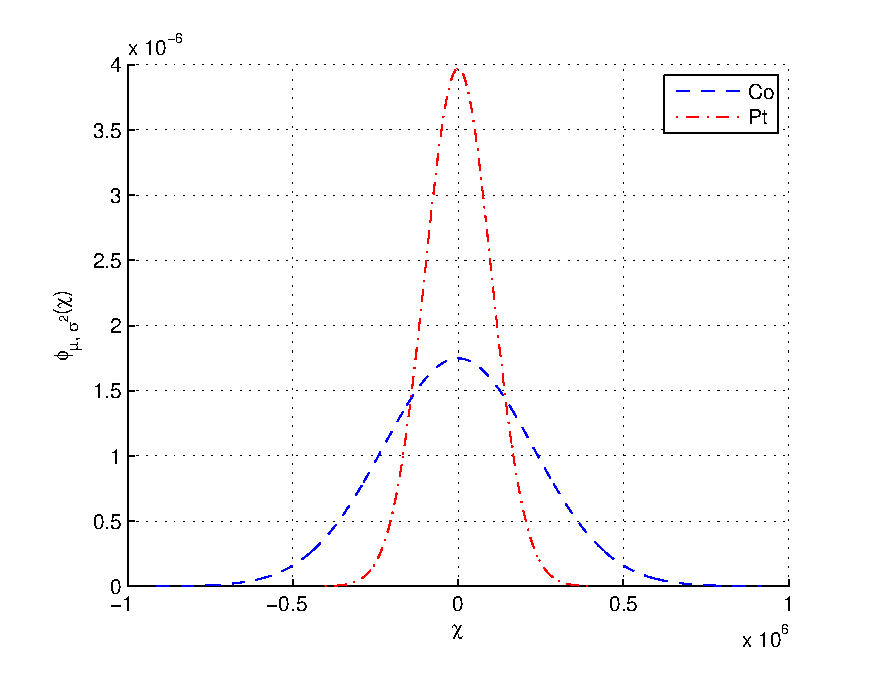
\includegraphics[width=250px]{figures/st_sw_linear_lda.eps}
  \caption{Kojos prisilietimo prie žemės ir pakilimo nuo žemės laiko
    variacijos pasiskirstymas po LDA transformacijos.}
  \label{fig:linear_lda}
\end{figure}

Sekantis metodas yra LDA. Transformacijos rezultatas yra pavaizduotas \ref{fig:linear_lda} pav. Kaip matosi - tiek po LDA, tiek po PCA duomenų pasiskirstymas nėra kritiškai skirtingas. Galima daryti hipotezę, kad linijinis duomenų praskirstymas šiuo atveju neveikia. Reikia taikyti branduolio metodą ir papildyti jau panaudotus transformacijos metodus polinominiu arba Gausso branduoliu.

\begin{figure}[!t]
  \centering
  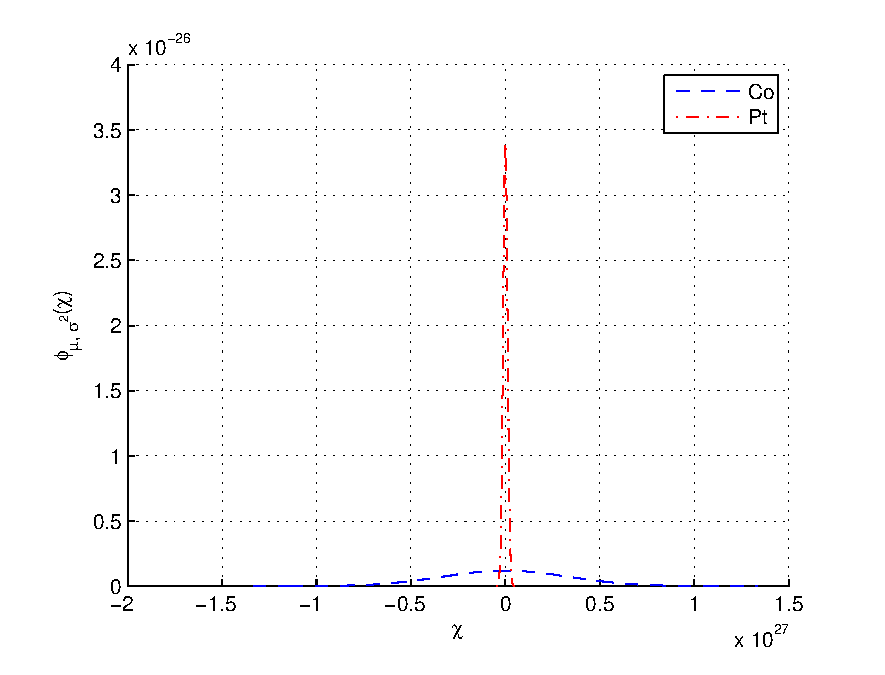
\includegraphics[width=250px]{figures/st_sw_poly_kpca.eps}
  \caption{Kojos prisilietimo prie žemės ir pakilimo nuo žemės laiko
    variacijos pasiskirstymas po PCA transformacijos, naudojant
    polinominį branduolį.}
  \label{fig:poly_pca}
\end{figure}

\begin{figure}[!t]
  \centering
  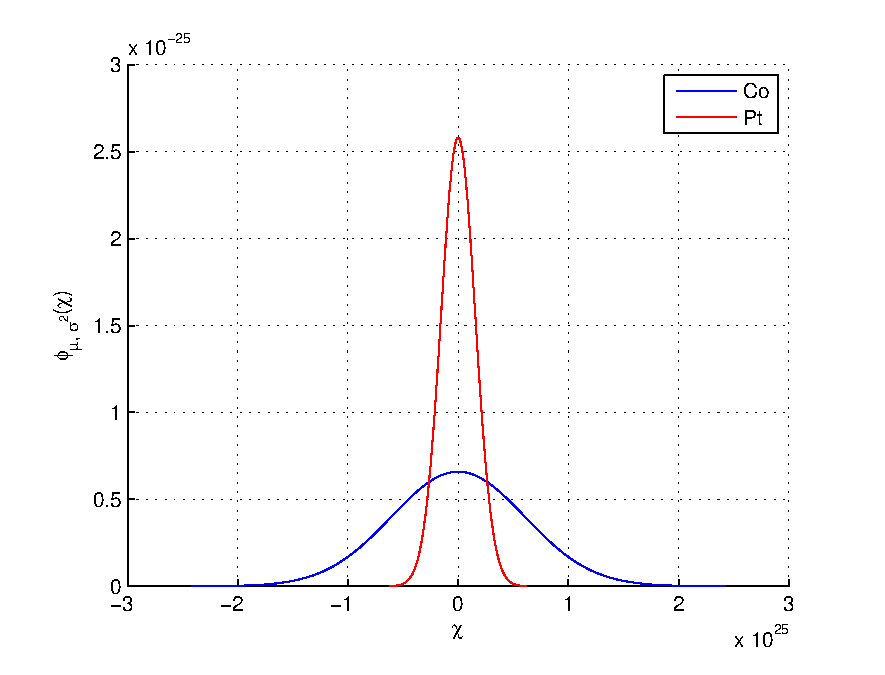
\includegraphics[width=250px]{figures/st_sw_poly_gda.eps}
  \caption{Kojos prisilietimo prie žemės ir pakilimo nuo žemės laiko
    variacijos pasiskirstymas po LDA transformacijos, naudojant
    polinominį branduolį.}
  \label{fig:poly_lda}
\end{figure}

\begin{figure}[!t]
  \centering
  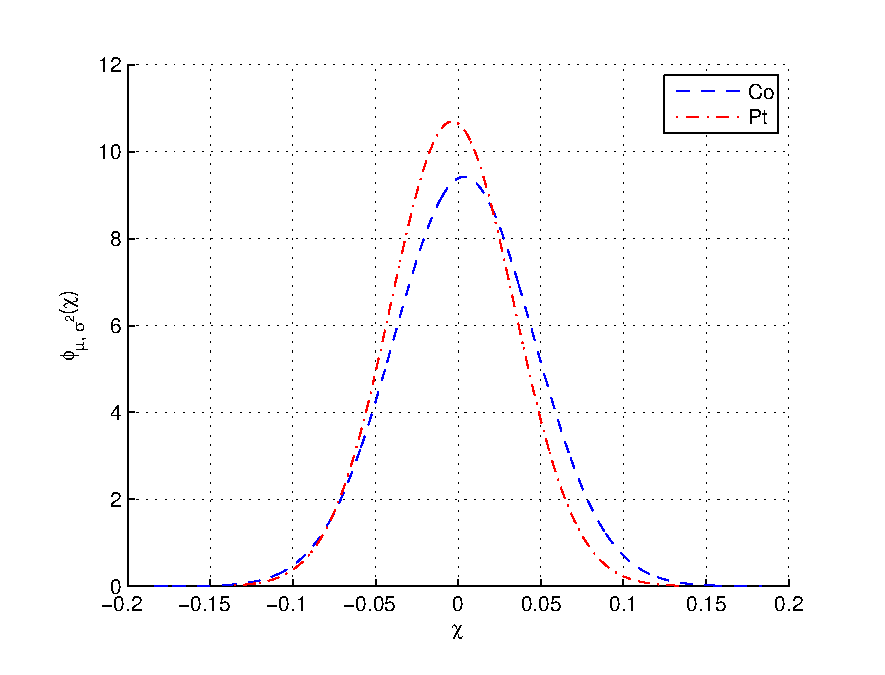
\includegraphics[width=250px]{figures/st_sw_gauss_kpca.eps}
  \caption{Kojos prisilietimo prie žemės ir pakilimo nuo žemės laiko
    variacijos pasiskirstymas po PCA transformacijos, naudojant Gauso branduolį.}
  \label{fig:gauss_pca}
\end{figure}

\begin{figure}[!t]
  \centering
  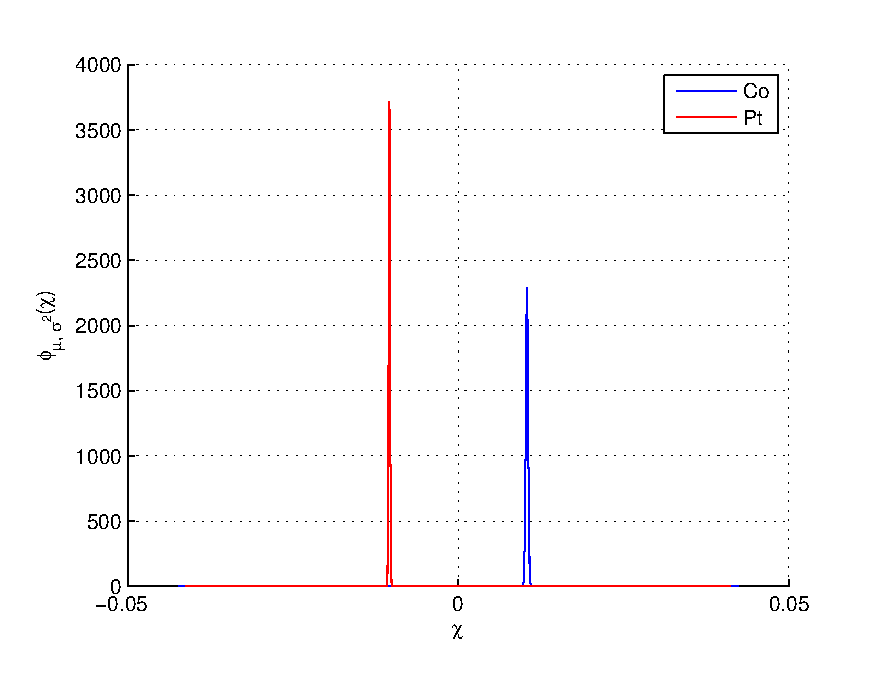
\includegraphics[width=250px]{figures/st_sw_gauss_gda.eps}
  \caption{Kojos prisilietimo prie žemės ir pakilimo nuo žemės laiko
    variacijos pasiskirstymas po LDA transformacijos, naudojant Gauso branduolį.}
  \label{fig:gauss_lda}
\end{figure}

Branduolio metodas pritaikytas PCA transformacijai yra pavaizduotas \ref{fig:poly_pca} pav. ir \ref{fig:gauss_pca} pav. Branduolio metodas pritaikytas LDA transformacijai yra pavaizduotas \ref{fig:poly_lda} pav. ir \ref{fig:gauss_pca} pav. Polinominis branduolys abiems atvejais buvo panaudotas su 4 branduolio argumentu.

Kaip matosi, panaudojus polinimonį branduolį, tiek PCA (\ref{fig:poly_pca} pav.), tiek LDA (\ref{fig:poly_lda} pav.) atveju - vidurkis iš savo vietos nepajudėjo. Abidvi transformacijos pakeitė variaciją. Tai nėra norimas tikslas, todėl toks branduolys nėra tinkamas. Panaudojus Gauso branduolį rezultatas labai pagerėja LDA transformacijos atveju (\ref{fig:gauss_lda} pav.), PCA su tokiu branduoliu (\ref{fig:gauss_pca} pav.) duomenis tik dar labiau suvienodina.

Remiantis pateikta analize galima teigti, kad geriausiai duomenis savybių erdvėje atskiria LDA su Gauso branduoliu. Tolimesniame darbe duomenis į klasifikatorių bus pateikiami būtent po tokios transformacijos.

\subsection{Požymių klasifikavimo programos kūrimas}

Šiame skyriuje bus išnagrinėti ir pritaikyti populiariausi šiuo metu naudojami klasifikatorių metodai. Tokie klasifikatoriai yra \cite{824819}:

\begin{itemize}
\item Vektoriaus palaikymo mašina (angl. Support Vector Machine (SVM));
\item Paslėptas Markovo modelis (angl. Hidden Markov Model (HMM));
\item Naivusis Bayes klasifikatorius (angl. NayveBayes);
\item Tiesioginio sklidimo neuronų tinklas (angl. Feed-Forward Neural Network (FFNN));
\end{itemize}

Labai svarbu yra atskirti duomenis, kuriais klasifikatorius yra apmokamas ir kuriais jis yra testuojamas. Jeigu klasifikatoriaus apmokymo duomenys yra pakankamai apibendrinti, tuomet naujus duomenis klasifikatorius turėtų gerai atpažinti. Pateikiant klasifikatoriaus testavime tokius pačius duomenis, kaip ir apmokyme - atliekamas tikrinimas ar klasifikatorius teisingai ``suprato'' nagrinėjamus duomenis, tačiau tai neapibrėžia kiek gerai jis apdoros naujus duomenis.

Nurodytų klasifikatorių veikimas bus vertinamas taiklumo ir tikslumo parametrais. Taiklumas apskaičiuojamas:

\begin{equation}
Taiklumas = \frac{T_P + T_N}{T_P + F_P + T_N + F_N},
\end{equation}
kur $T_P$ - teisingai identifikuotų klasių skaičius, $T_N$ - teisingai atmestų klasių skaičius, $F_P$ - klaidingai identifikuotų klasių skaičius ir $F_N$ - klaidingai atmestų klasių skaičius.

Tikslumas apskaičiuojamas:

\begin{equation}
Tikslumas = \frac{T_P}{T_P + F_P}
\end{equation}

Visos tolesnės klasifikatorių patikros bus atliekamos remiantis tokia schema: iš turimų duomenų buvo išskirta kojos prisilietimo ir pakilimo nuo žemės laiko ilgio variacijos savybė. Tuomet visi duomenys buvo padalinti į lygias tris dalis: dimensijų operacijai atlikti buvo duota $500$ reikšmių, klasifikatoriaus apmokymui $500$ verčių, klasifikatoriaus testavimui $500$ verčių. Klasifikavimas buvo atliekamas realiu laiku, t.y. klasifikatoriui pateikiami duomenis apie žingsnio stadijos variaciją po transformacijos ir klasifikatorius pateikia savo spėjimą.

Vektoriaus palaikymo mašina \cite{Burges98atutorial} šiuo metu yra populiariausias klasifikatorius nagrinėjant netiesiškai atskiriamus duomenis. Įgyvendinimas Matlab aplinkoje buvo panaudotas iš \cite{website:svm_implementation}. Klasifikatoriaus testavimo metu buvo naudojami tokie parametrai:

\begin{itemize}
\item SVM tipas - Siquential Minimal Optimization;
\item Branduolio tipas - linijinis;
\item Sureguliavimo konstanta - 2;
\item Branduolio argumentas - 2;
\end{itemize}

Lentelėje \ref{table:svm_scores} pateikti SVM tikslumo ir taiklumo duomenis. Kaip matosi, klasifikatorius veikia nepakankamai gerai - tikslumo koeficientas nėra didesnis negu pusę, abiems atvejams tik $0.489$. Pirmos klasės atpažinimo taiklumas tėra $0.234$, antros klasės atpažinimo taiklumas yra $0.744$, tačiau to nepakanka. Iš padarytos klasifikatoriaus veikimo analizės galima teigti, kad klasifikatorius veikia blogai ir jo naudoti sprendime nėra galima.

\begin{table}[!t]
  \centering
  \caption{Vektoriaus palaikymo mašinos tikslumas ir taiklumas.}
  \label{table:svm_scores}
  \begin{tabular}{|c|c|c|} \hline
    & Co & Pt \\ \hline
    Tikslumas & 0.489 & 0.489 \\ \hline
    Taiklumas & 0.234 & 0.744 \\ \hline
  \end{tabular}
\end{table}

Paslėptas Markovo modelis \cite{18626} yra vienintelis iš šiame darbe nagrinėjamų klasifikatorių, kuris turi laikinę informaciją. Tokia savybė suteikia ``inkaro'' galimybę - klasifikatorius gali užsilaikyti prie vienos klasės net ir tuomet, kai pagal savybių erdvę turi būti kitas klasifikavimo rezultatas. Tokia klasifikatoriaus savybė buvo pritaikyta ankstesniame darbe, sudarant žmogaus eisenos atpažinimo sprendimą \cite{mano_darbas}. Pasirinktas modelis, susidedantis iš dviejų būsenų - ``Sveikas'', ``Sergantis''. Būsenos tarpusavyje yra sujungtos (\ref{fig:hmm_model} pav.). Perėjimo tikimybės tarp modelio elementų buvo parinktos žymiai mažesnės už tikimybę likti toje pačioje būsenoje. Įgyvendinimas Matlab aplinkoje buvo panaudotas iš \cite{website:hmm_implementation}.

\begin{figure}
	\centering
	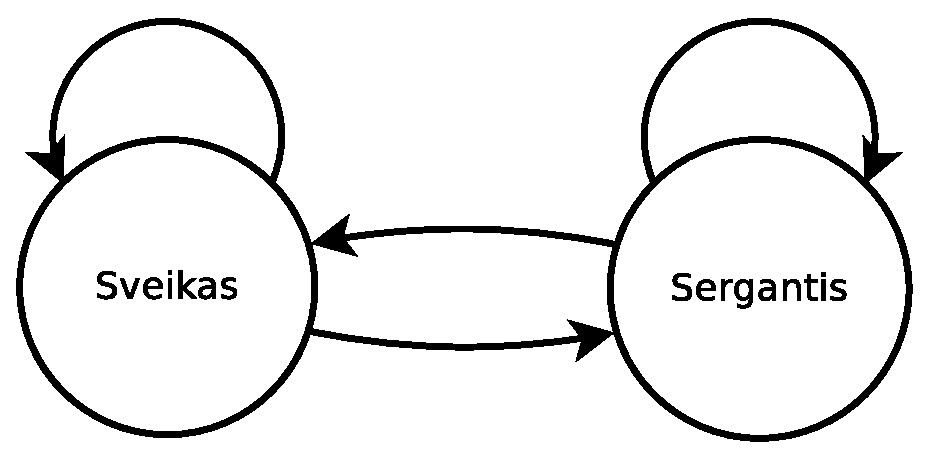
\includegraphics[width=250px]{figures/hmm_modelis}
	\caption{Ergodinis paslėptas Markovo modelis}
	\label{fig:hmm_model}
\end{figure}

Lentelėje \ref{table:hmm_scores} pateikti tikslumo ir taikumo duomenys. Kaip matome iš tikslumo rezultato - klasifikatorius teisingai priskiria tik pusei reikiamų duomenų. Iš to galime teigti, kad klasifikatorius yra labai blogai apmokytas ir visiškai nesugeba apibendrinti turimų duomenų. Klasifikatorius visus pateikiamus testavimo duomenis priskiria vienai klasei.

\begin{table}[!t]
  \renewcommand{\arraystretch}{1.3}
  \centering
  \caption{Paslėpto Markovo modelio tikslumas ir taiklumas.}
  \label{table:hmm_scores}
  \begin{tabular}{|c|c|c|} \hline
    & Co & Pt \\ \hline
    Tikslumas & 0.500 & 0.500 \\ \hline
    Taiklumas & 0.000 & 1.000 \\ \hline
  \end{tabular}
\end{table}

Naivus Bayes \cite{R22230} yra vienas iš pirmųjų statistinių metodu paremtu klasifikavimo mechanizmas. Jis veikia labai paprastai - ieškoma linijinės funkcijos, kuri geriausiai atskiria nagrinėjamus duomenis ir vieni žymenis priskiriami, jeigu duomenys yra vienoje linijos pusėje, atvirkšti žymenis priskiriami, jeigu duomenys yra kitoje linijos pusėje. 

Lentelėje \ref{table:nb_scores} pateikti tikslumo ir taiklumo duomenys. Tikslumo koeficientas viršija pusę, $0.508$, tačiau tai yra mažai. Taiklumo koeficientas pirmuoju atveju yra neblogas, $0.764$, tačiau antruoju atveju koeficientas yra visiškai nepatenkinamas, viso $0.252$. Iš turimų rezultatų galima teigti, kad klasifikatorius veikia blogai ir duomenis vienmatėje erdvėje jis klasifikuoti teisingai negali.

\begin{table}[!t]
  \centering
  \caption{Naivaus Bayes klasifikatoriaus tikslumas ir taiklumas.}
  \label{table:nb_scores}
  \begin{tabular}{|c|c|c|} \hline
    & Co & Pt \\ \hline
    Tikslumas & 0.508 & 0.508 \\ \hline
    Taiklumas & 0.764 & 0.252 \\ \hline
  \end{tabular}
\end{table}

Paskutinis klasifikatorius, kuris bus pritaikytas esamiems duomenims - tiesioginio sklidimo neuronų tinklas. Tai yra dirbtinių neuronų tinklų klasifikatorius, kuris veikia panašiai kaip ir Naivus Bayes - jis ieško funkcijos (linijinės arba polinominės), kuri geriausiai atskiria turimus duomenis. Bandymo metu buvo pasirinktas vienas įėjimas, du išėjimai ir vienas paslėptas sluoksnis. 

Lentelėje \ref{table:ffn_scores} pateikiami tiesioginio sklidimo dirbtinių neuronų tinklų tikslumas ir taiklumas. Kaip matosi iš rezultatų - klasifikatoriaus tikslumas pirmos klasės atžvilgiu yra $0.282$, taiklumas $0.000$, antros klasės atžvilgiu klasifikavimo tikslumas yra artimas pirmai $0.287$, tačiau turi geresnį taiklumą $0.392$. Iš turimos patikros rezultatų galima spręsti, kad tiesioginio sklidimo neuronų tinklas užduotį atlieka blogai.

\begin{table}[!t]
  \centering
  \caption{Tiesioginio sklidimo dirbtinių neuronų tinklų tikslumas ir taiklumas.}
  \label{table:ffn_scores}
  \begin{tabular}{|c|c|c|} \hline
    & Co & Pt \\ \hline
    Tikslumas & 0.282 & 0.287 \\ \hline
    Taiklumas & 0.000 & 0.392 \\ \hline
  \end{tabular}
\end{table}

Iš pateiktos analizės galima spręsti, kad realiu laiku pateikti klasifikavimo rezultatai nėra pakankamai geri, norint atlikti kokybišką spėjimą ligos atžvilgiu. Vektoriaus palaikymo mašinos tikslumas neviršija pusės, paslėptas Markovo modelis nesugeba atlikti tikslingo apmokymo, naivus Bayes klasifikatorius užduotį atlieka geriausiai iš visų nagrinėjamų klasifikatorių, tiesioginio sklidimo neuronų tinklas užduotį atlieka blogiausiai, iš visų klasifikatorių, kurie sugebėjo bent kažkiek apibendrinti duodamus duomenis apmokymo metu. Atlikta analizė reikalauja kito būdo klasifikavimui atlikti. Naudojamas būdas bus aprašytas sekančiame poskyryje.

\subsection{Duomenų analizės programos kūrimas}

Šiame poskyryje bus aptartas duomenų analizės programos kūrimas. Pasinaudojus prieš tai esančių skyrių informacija bus pateiktas sprendimas, kuris leidžia efektyviai kiek įmanoma efektyviau atpažinti subjektų tipus.

Poskyryje ``Požymių išskyrimo programos kūrimas'' buvo atlikta savybių ir dimensijų mažinimo metodų analizė. Geriausia savybė, kuri atskiria kontrolinį subjektą nuo Parkinsono subjekto yra kojos pakilimo ir prisilietimo prie žemės laiko variacija. Geriausiai dimensijų mažinimo klausimą išsprendė linijinė diskriminanto analizė, naudojant Gauso branduolį, tačiau iškilo klasifikavimo problema - klasifikuojant duomenis realiu laiku, klasifikavimo rezultatas buvo nepatenkinamas. 

Pagrindinė problema, kodėl joks nagrinėjamas klasifikatorius neatliko korektiško klasifikavimo, tai dėl jam pateikiamų duomenų. Kaip pavyzdys yra pateikiamas klasifikatoriaus testavimo metu naudoti duomenis, pavaizduoti \ref{fig:testing_sample} pav. Duomenis yra pateikiami po atliktos transformacijos, todėl jie yra vienos dimensijos. Horizontalėje yra pateiktas požymio eilės numeris, vertikalėje - pirmas LDA diskriminantas. Pirmi $500$ požymiai priklauso kontroliniam subjektui, nuo $501$ iki $1000$ požymiai priklauso Parkinsono subjektui. Lyginant matomus duomenis su jų pasiskirstymu \ref{fig:gauss_lda} pav., jie atrodo labiau chaotiški. Iš vaizdinės analizės nėra įmanoma spėti kuri signalo dalis kuriai subjektų grupei priklauso. 

\begin{figure}
	\centering
	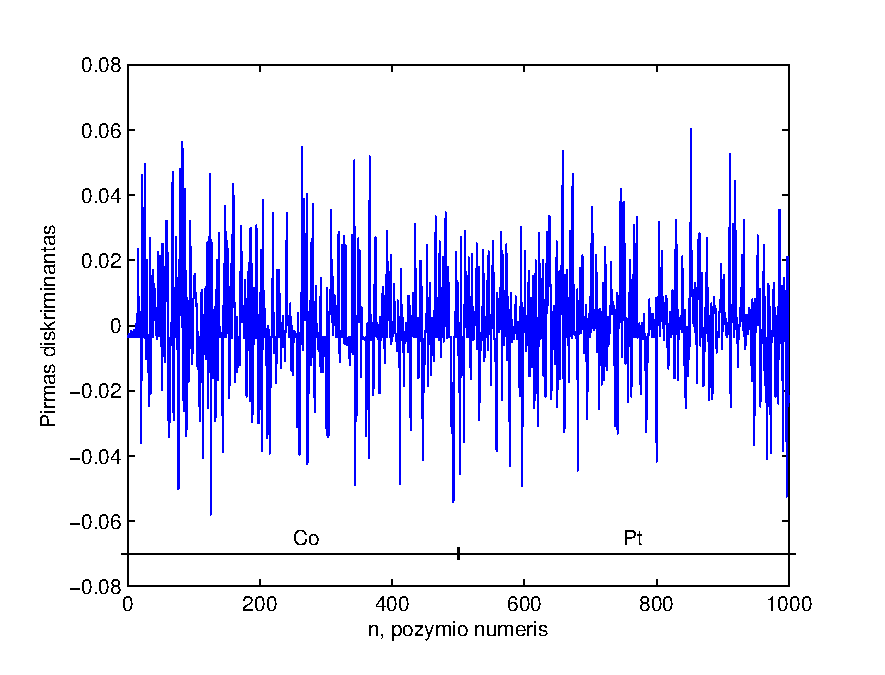
\includegraphics[width=250px]{figures/11_sample_testing}
	\caption{Kojos pakilimo ir kojos prisilietimo prie žemės ilgio variacijos kitimas slenkant langui, po transformacijos.}
	\label{fig:testing_sample}
\end{figure}

Tokios išvados verčia projektuoti kitą klasifikavimo mechanizmą, kuris duomenis klasifikuotų ne kiekvieną pagal kiekvieną nagrinėjamą savybę, o pagal savybės grupes - į laikiną atmintį yra rašoma požymio reikšmė, laukiama, kol laikina atmintis užsipildys iki tam tikros $n$ eilės ir iš gautos sekos yra skaičiuojamas vidurkis (vidurkis skaičiuojamas todėl, nes pagal duomenų pasiskirstymą, kuris parodytas \ref{fig:gauss_lda} pav., pasiskirstymų vidurkiai skiriasi, tačiau variacijos lieka tokios pačios) ir apskaičiuota reikmė naudojama kaip nauja savybė klasifikatoriaus apmokymui, bei testavimui. 

Dėl gaunamų duomenų dimensijos ir jų mažo kiekio (kuris priklauso nuo laikinos atminties dydžio, į kurią rašomos naudos erdvės vertės), bus panaudotas papraščiausias naivaus Bayes klasifikatoriaus mechanizmas. Dėl duomenų stokos, kai kurie duomenys buvo panaudoti visuose trijuose algoritmo veikimo žingsniuose. Viso erdvės sudarymui buvo panaudota $900$, apmokymui $500$, testavimui $700$ reikšmių. Laikinos atminties ilgis buvo pasirinktas $150$ verčių, iš kurių buvo skaičiuojamas vidurkis. Apmokymo metu iš viso buvo $3$ vidurkiai kiekvienai subjektų grupei, testavimo metu iš viso buvo $4$ vidurkiai kiekvienai subjektų grupei. Gauti rezultatai pateikti \ref{table:classification_results} lentelėje.

\begin{table}
	\centering
	\caption{Gautas klasifikavimo rezultatas, naudojant naivų Bayes klasifikatorių.}
	\label{table:classification_results}
	\begin{tabular}{|c|c|c|} \hline
		& Co & Pt \\ \hline
    Tikslumas & 0.800 & 0.800 \\ \hline
    Taiklumas & 0.714 & 1.000 \\ \hline
	\end{tabular}
\end{table}

Gauti klasifikavimo tikslumas yra $0.800$, kas viršija prieš tai naudotų metodų tikslumą. Pirmos grupės klasifikavimo tikslumas yra $0.714$, antros grupės klasifikavimo tikslumas $1.000$. Detalesnė klasifikavimo mechanizmo veikimo apžvalga yra pateikta Požymių klasifikavimo programos kūrimo poskyryje.

\section{Signalų analizės programos įgyvendinimas}

Šiame skyriuje bus apžvelgta įgyvendintas programinis kodas, jo veikimo architektūra. Ankstesniuose poskyriuose buvo argumentuotai pažvelgti galimi analizės metodai, požymiai ir klasifikatoriai. Visi rezultatai bus panaudoti projektuojant galutinį sprendimą.

Poskyryje \ref{subsec:total_scheme} bus pateikta bendra programos algoritmo veikimo schema, poskyryje \ref{subsec:class_scheme} bus pateikta algoritmo klasifikavimo veikimo schema, poskyryje \ref{subsec:total_program} bus apžvelgta galutinė programa.

\subsection{Bendro programos algoritmo schemos sudarymas}
\label{subsec:total_scheme}

Ankstesniame skyriuje buvo apžvelgta bendra programos veikimo schema. Bendros schemos pavyzdys yra pateiktas \ref{fig:pirmine_programos_schema} pav. Šiame  poskyryje bus patekta detali algoritmo schema ir aptarta kiekviena jo bloko paskirtis, bei jame naudojamas metodas.

Viso programa yra sudaryta iš trijų modulių:

\begin{itemize}
\item Savybių erdvės sudarymas;
\item Klasifikatoriaus apmokymas;
\item Klasifikatoriaus tikrinimas.
\end{itemize}

\begin{figure}[!t]
  \centering
  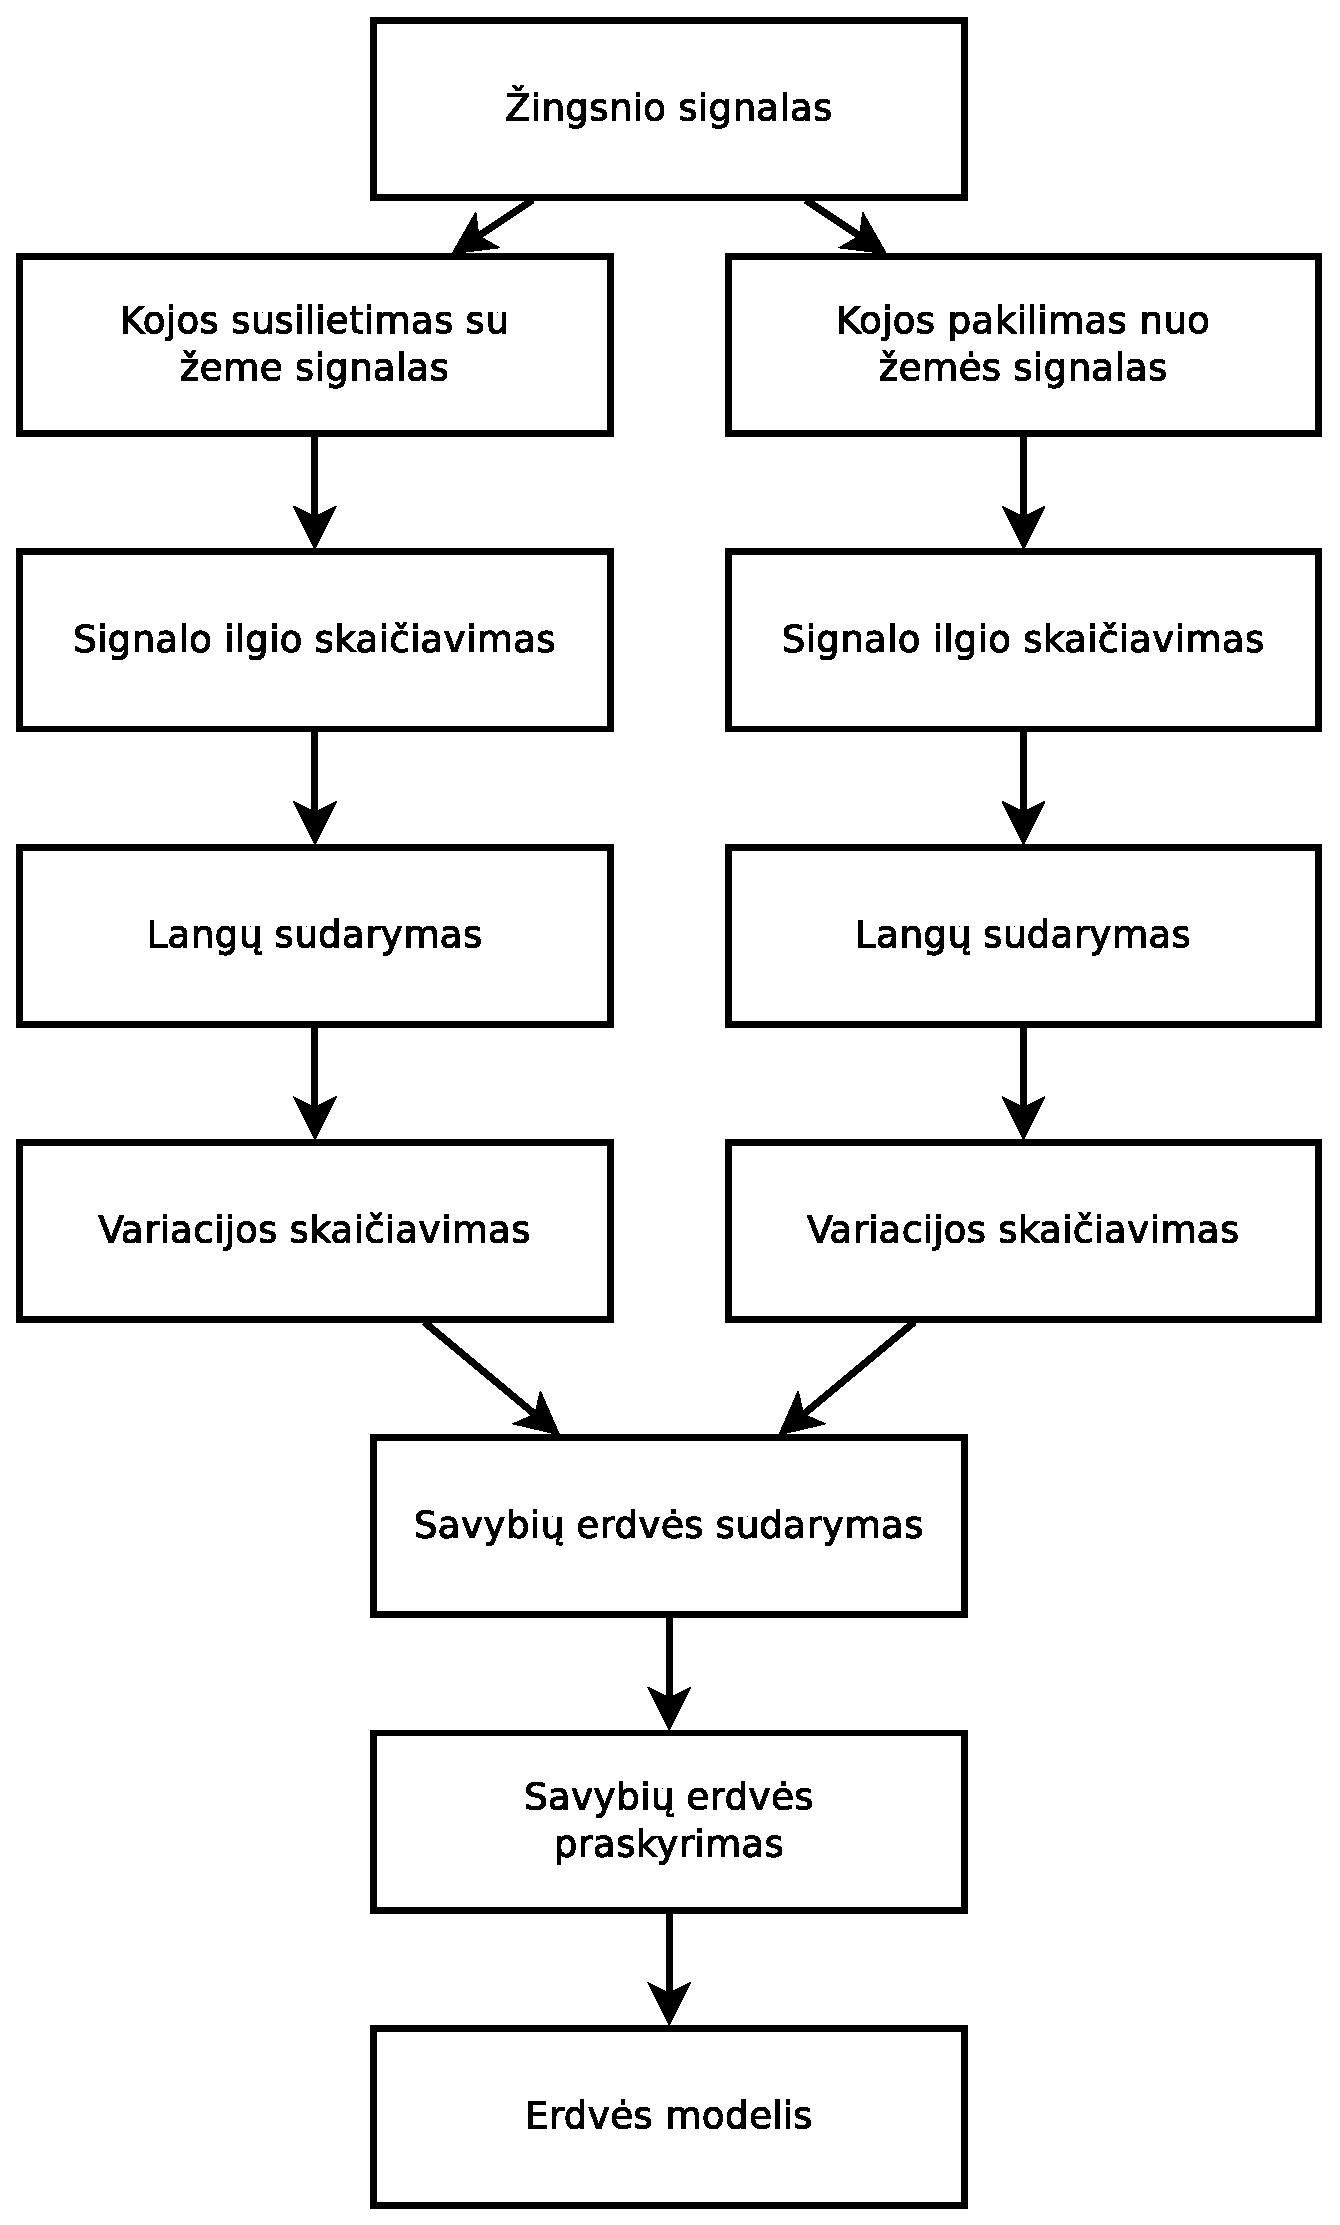
\includegraphics[width=250px]{figures/pirma_faze.eps}
  \caption{Programos pirmo modulio grafikas.}
  \label{fig:pirma_faze}
\end{figure}

\begin{figure}[!t]
  \centering
  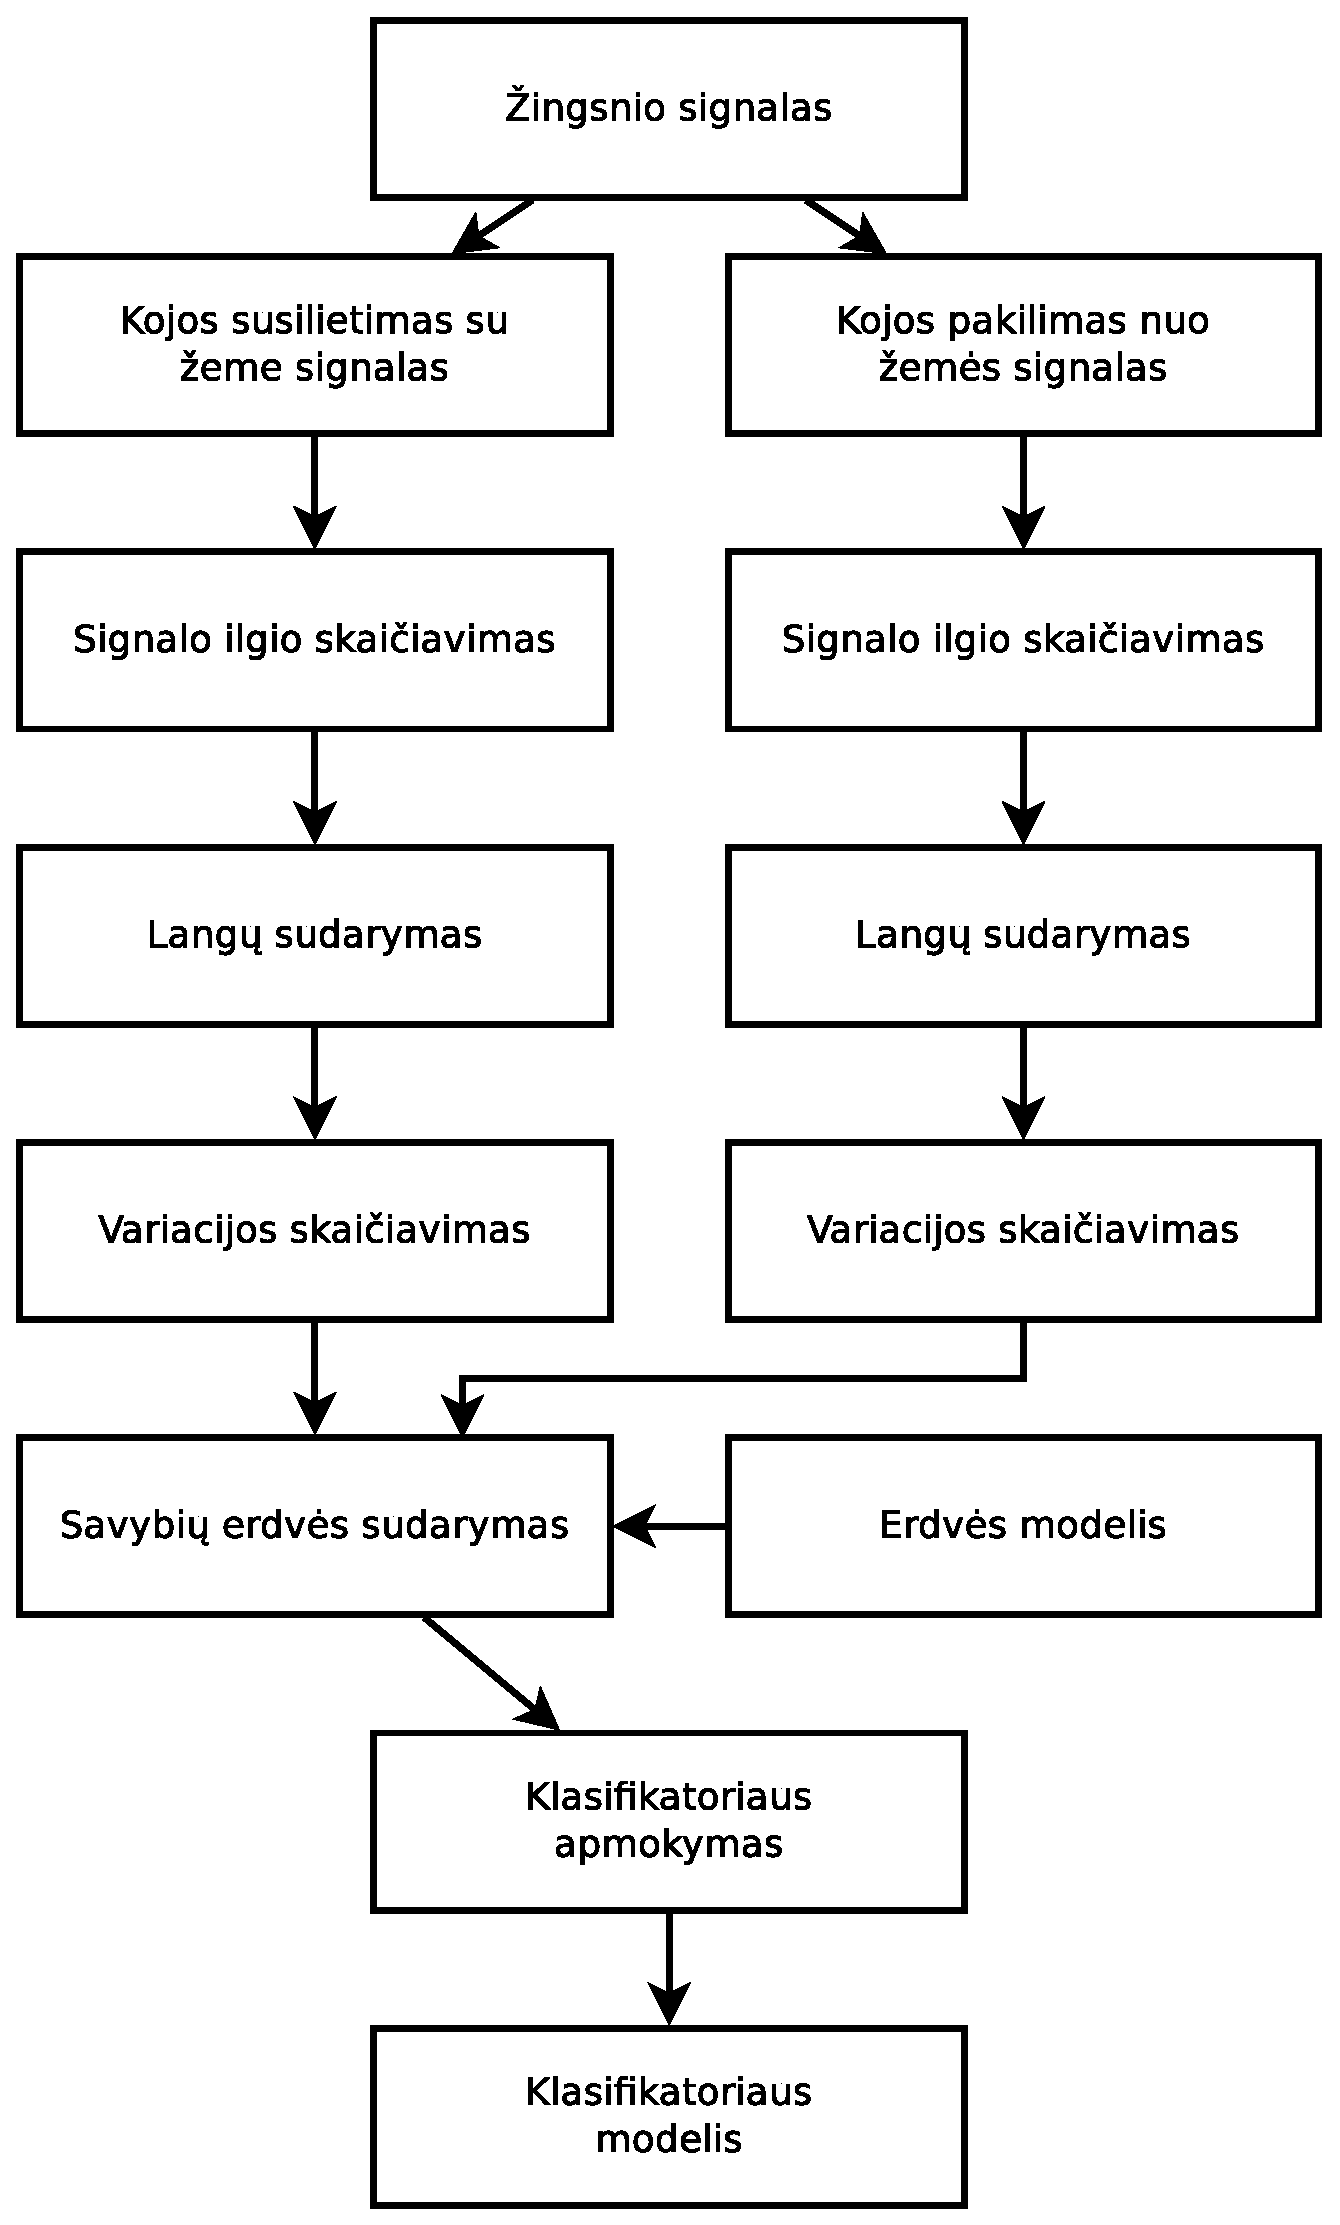
\includegraphics[width=250px]{figures/antra_faze.eps}
  \caption{Antro modulio grafikas.}
  \label{fig:antra_faze}
\end{figure}

\begin{figure}[!t]
  \centering
  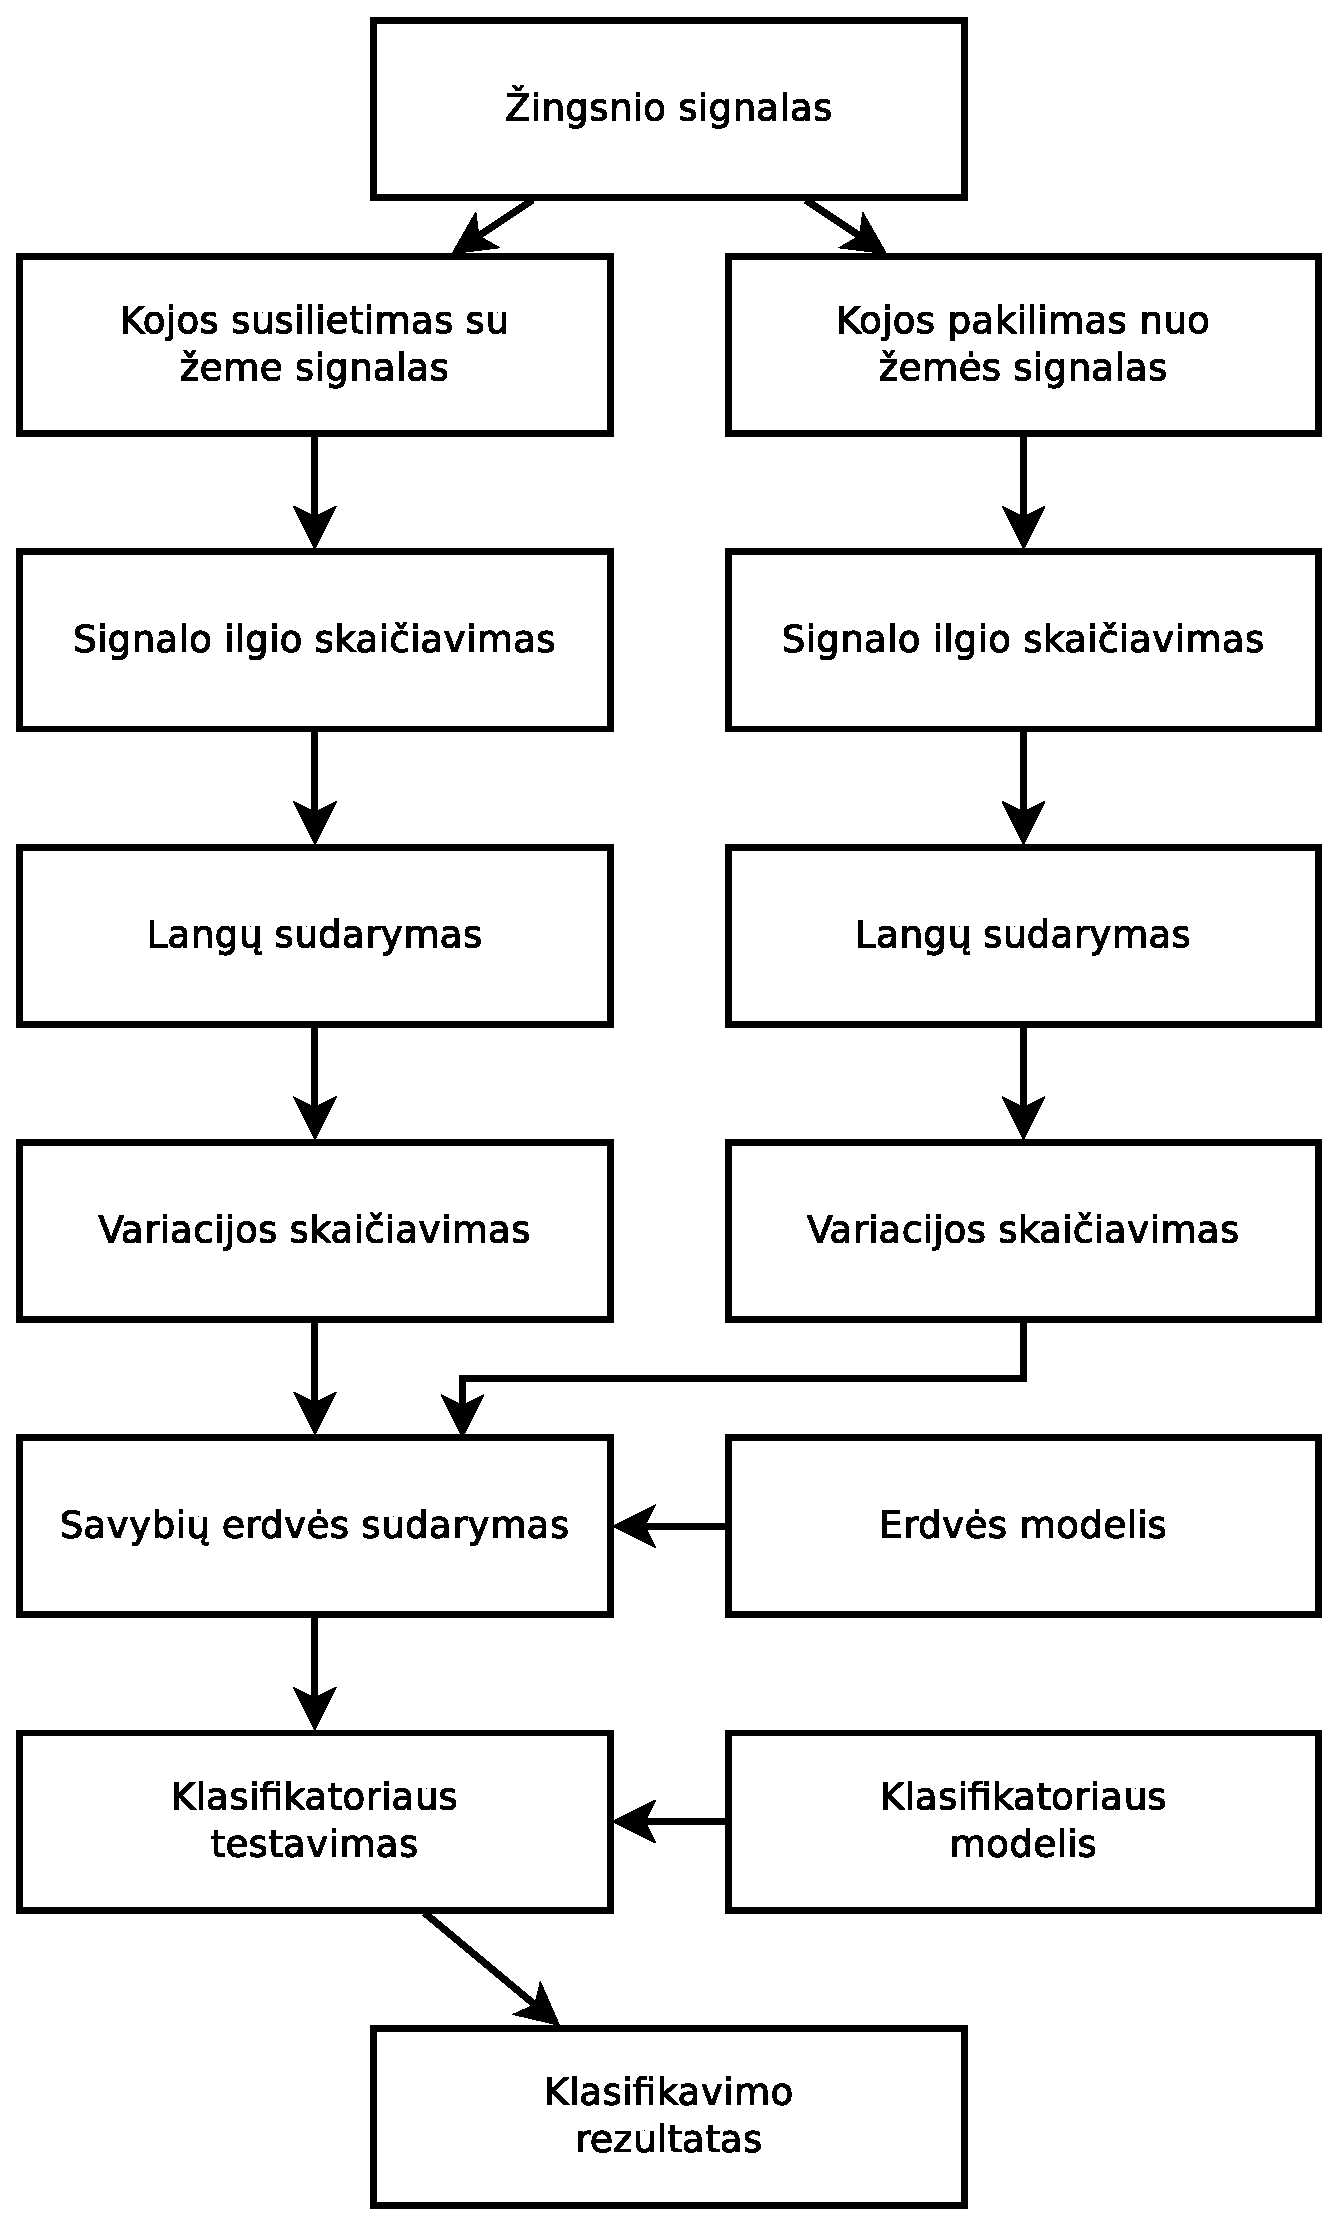
\includegraphics[width=250px]{figures/trecia_faze.eps}
  \caption{Trečio modulio grafikas.}
  \label{fig:trecia_faze}
\end{figure}

Programos pirmo modulio struktūrinė schema pavaizduota \ref{fig:pirma_faze} pav. Programos įėjime yra pateikiami pirminiai žingsnio duomenys, programa lygiagrečiai iš duomenų išskiria kojos susilietimo su žeme ir kojos pakilimo nuo žemės signalus, paskaičiuoja signalų ilgius, iš signalų ilgių sudaro duomenų langus, paskaičiuoja lange esančių signalų variacijos koeficientą. Toliau programa iš esamų dviejų dimensijų sudaro savybių erdvę, pritaiko LDA transformacija su Gauso branduoliu ir gražina erdvės modelį, kuris susideda iš tikrinio vektoriaus ir duomenų vidurkio.

Programos antro modulio struktūrinė schema pavaizduota \ref{fig:antra_faze} pav. Struktūroje naudojamas erdvės modelis iš pirmojo programos modulio. Jis reikalingas tam, kad kiekvieną kartą neprojektuoti naujos erdvės iš naujo, bet projektuoti naujus duomenis į jau esamą erdvę. Tai taip pat užtikrina, kad bus naudojama ta pati erdvė, kas leidžia užtikrinti duomenų apibendrinimą. Sistemos įėjimas yra toks pats, kaip ir pirmojo modulio. Skirtumas taip pirmojo ir antrojo modulio yra tas, kad antro modulio išėjime yra klasifikatoriaus modelis, kuris yra apmokyto klasifikatoriaus parametrai, kurie bus panaudoti testuojant klasifikatorių.

Trečiojo, paskutinio modulio, struktūrine schema pavaizduota \ref{fig:trecia_faze} pav. Struktūroje naudojamas erdvės modelis iš pirmo modulio ir klasifikatoriaus modelis iš antro modulio. Modulio įėjimas yra toks pats, kaip ir antrojo modulio, išskyrus tai, kad šio modulio išėjime yra klasifikavimo rezultatas, kurį galima pateikti tiek grafiškai, tiek skaitine išraiška, išreikšta tikslumo ir taiklumo verte.

Apibendrinus bendrą programos veikimo schemą, toliau paanalizuosim patį klasifikavimo mechanizmą - naivųjį Bayes klasifikatorių.

\subsection{Požymių klasifikavimo programos algoritmo schemos sudarymas}
\label{subsec:class_scheme}

Šiame poskyryje bus apžvelgtas naudojamas klasifikatorius, trumpai apžvelgtas jo veikimo principas, bei įgyvendinimas.

Naivus Bayes klasifikatorius \cite{R22230} yra paprastas tikimybinis klasifikatorius, kuris paremtas Bayes teorema su stipria duomenų nepriklausomybės prielaida, kuri išreiškiama:

\begin{equation}
	P(\mathbf{X}|C) = \prod_{i=1}^{n} P(X|C),
\end{equation}
kur $\mathbf{X} = (X_1, \cdot \cdot \cdot, X_n)$ yra savybių vektorius, o $C$ yra klasės identifikatorius. Nepriklausomai nuo to, kad tokia duomenų atskyrimo prielaida yra labai naivi - praktikoje metodas veikia pakankamai gerai, ir yra naudojamas daugelį sudėtingesnių metodikų.

Bayes klasifikatorius $h^*(x)$, naudoja diskriminanto funkcijas atnaujinti klasės vėlesnes tikimybes, nurodant savybių vektorių:

\begin{equation}
	f^*_i(x) = P(C=i|\mathbf{X}=x).
\end{equation}

Pritaikius Bayes taisyklę nurodytai lygčiai, gaunamas rezultatas:

\begin{equation}
P(C=i|\mathbf{X}=x) = \frac{P(\mathbf{X}=x|C=i)P(C=i)}{P(\mathbf{X}=x)},
\end{equation}
kur $P(\mathbf{X}=x)$ yra identiška visoms klasėms, todėl yra ignoruojama. Iš to seka Bayes diskriminato funkcija:

\begin{equation}
	f^*_i(x) = P(\mathbf{X}=x|C=i)P(C=i),
\end{equation}
kur $P(\mathbf{X}=x|C=i)$ vadinama klasės priklausomybės tikimybės pasiskirstymas. Taigi, Bayes klasifikatorius:

\begin{equation}
h^*(x) = arg max_i P(\mathbf{X}=x|C=i)P(C=i)
\end{equation}
randa didžiausią vėlesnės tikimybės hipotezę, nurodžius $x$.

Duomenys Hilberto erdvėje yra labai gerai praskiriami linijine funkcija, todėl šiame sprendime yra naudojamas tokios paprastos struktūros klasifikavimo mechanizmas. Tuo labiau, kadangi duomenis yra vienmatėje erdvėje - mažinti dimensijų skaičių nelieka prasmės, ieškoti klasifikavimo algoritmo, kuris geriausiai apibendrintų turimus duomenis erdvėje nėra prasmės, kadangi duomenų apibendrinimą puikiausiai atliko LDA su Gauso branduoliu.

Darbe bus panaudota Matlab aplinkoje įgyvendintas naivaus Bayes klasifikatoriaus versija, kuri yra ``Statistical Toolbox'' paketo dalis.

\subsection{Signalų analizės programos įgyvendinimas}
\label{subsec:total_program}

Šiame skyriuje apžvelgsime jau galutinę programą, aptarsime jos pritaikymo problemas, bei galimas pritaikymo platformas.

\begin{figure}[!t]
  \centering
  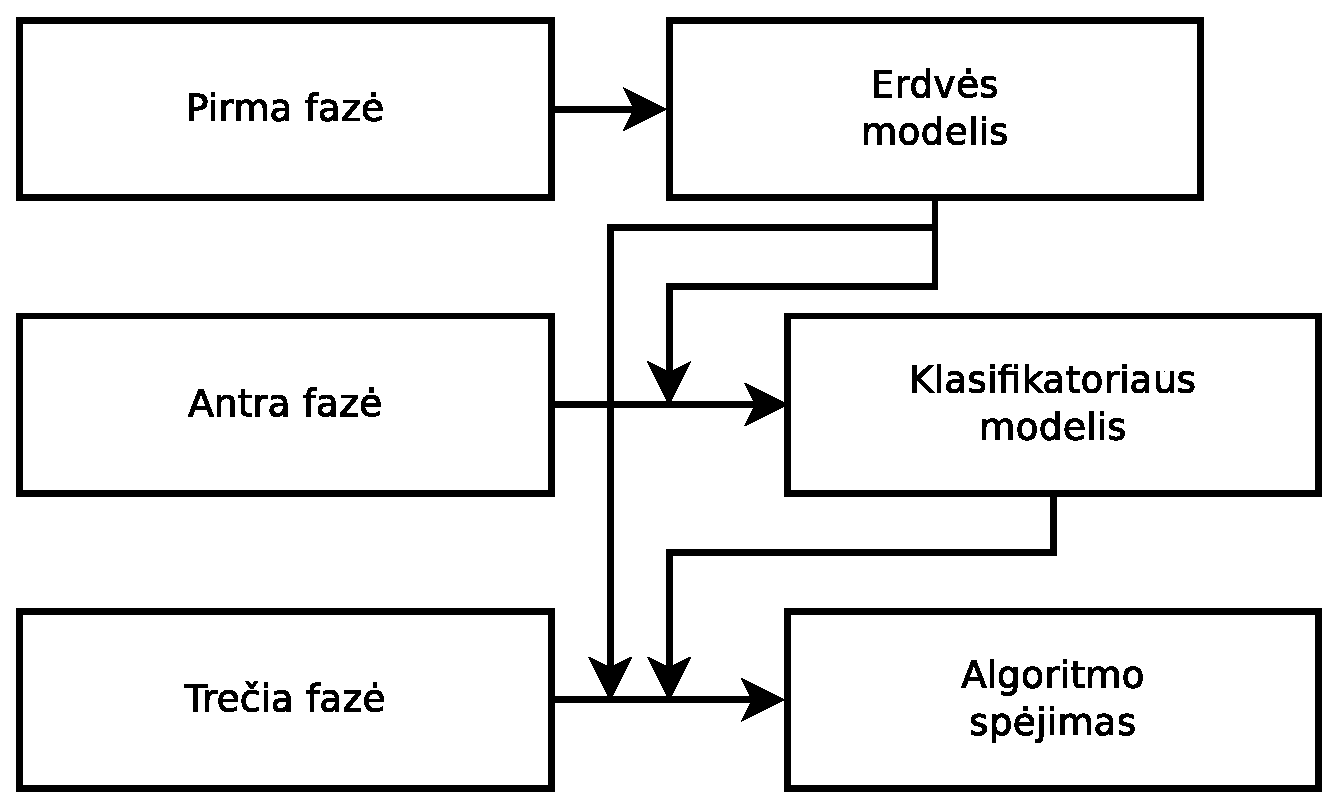
\includegraphics[width=250px]{figures/galutine_programa.eps}
  \caption{Galutinės programos struktūrinė schema.}
  \label{fig:galutine_programa}
\end{figure}

Galutinė programos schema yra pavaizduota \ref{fig:galutine_programa} pav. Kaip buvo aptarta ankstesniuose poskyriuose - programa susideda iš trijų duomenų apdorojimo modulių. Kiekvieno modulio įėjimas yra toks pats, tačiau kiekvieno modulio išėjimas yra skirtingas. Kiekvienas žemiau esantis modulis naudoja virš jos esančio modulio darbo rezultatą. Kritiškai svarbu yra kiekvienam moduliui pateikti skirtingus duomenis.

Darbe pateiktas metodas leidžia efektyviai atpažinti ar subjektas serga Parkinsono liga. Didžiausias metodo trūkumas yra tas, kad ji neatsižvelgia į kitus Parkinsono ligos simptomus - drebulys, eisenos sustingimas. Nurodytas trūkumas yra planuojamas pašalinti vėlesnėse darbo versijose, kurios bus kuriamos po pateikto darbo įgyvendinimo.

Drebulys gali pasireikšti ne tik plaštakos raumenyse, tačiau ir kaklo srityje. Tai neleidžia tiksliai apibrėžti kurią kūno vietą reikia stebėti ir rinkti duomenis tyrimui. Eisenos sustingimas taip pat yra sunkiai apibrėžtas faktorius, kadangi jo aptikimas yra labai didelis iššūkis signalų apdorojimo srityje. Geriausią ką šiuo metu gali pasiūlyti mokslas, stebint tokius ligos simptomus - paciento stebėjimas kameros pagalba, jo veiklos automatinis nustatymas. Drebulys subjektui dažniausiai pasireiškia, kai jo kūnas yra visiškai atsipalaidavęs, t.y. kai subjektas stovi, sėdi, guli, kai jis išlaiko statišką poziciją, tuomet pasireiškia drebulys. Kameros pagalba galima nustatyti kokioje pozicijoje yra subjektas, tačiau identifikuoti drebulį yra labai sudėtinga, jeigu naudojama kamera yra mažos rezoliucijos. Drebulį veiklos nustatymo algoritmas gali palaikyti tiesiog pašaliniu triukšmu, kaip šešėlio sudarymą ant stebimo paviršiaus. 

Darbas ties Parkinsono ligos identifikavimu ir jo diagnozavimui reikia įdėti dar daug darbo, tačiau besivystant kompiuteriniai technikai, bei atsirandant vis naujiems algoritmams nestandartinėms problemoms spręsti - šansas, kad ateityje šios ligos diagnozavimas pagerės, išlieka labai didelis.

\section{Signalų analizės programos patikra}

Šiame skyriuje bus parengtas ir įgyvendintas algoritmo patikros planas. Programos patikra yra kritinis aspektas jos patikimumo tikrinimui. Algoritmą galima tikrinti mažinant apmokymo verčių skaičių ir didinant tikrinimo verčių kiekį - taip bus sužinota kiek mažiausiai verčių reikia metodui, norint pilnai apibendrinti turimus duomenis.

Tikrinant kiekvieno žmogaus žingsnio signalus, paaiškėjo, kad skirtingi subjektai sugeneruoja kitokį tikrinimą atliktų žingsnių skaičių, todėl tikrinimas bus atliekamas ne atskiriant konkrečius žmones, tačiau jau išskirtus kojos pakilimo ir kojos prisilietimo prie žemės signalus, konkrečiau - iš tų signalų suformuotus jų ilgių duomenų langus.

Po pirminio duomenų apdorojimo, kontrolinių subjektų grupėje liko $1790$ duomenų langų, Parkinsono subjektų grupėje liko $1619$ duomenų langų, todėl buvo nuspręsta iš kiekvienos grupės pasiimti po $1500$ langų duomenų, visi jie padalinti po lygias tris dalis: viena dalis erdvės sudarymui, antra dalis klasifikatoriaus apmokymui, trečia dalis klasifikatoriaus testavimui. Jokie duomenys jokioje dalyje pasikartotinai nesikartoja. Tai yra kritinis faktorius mašininiam apmokyme \cite{824819}. Taip pat reikia užtikrinti duomenų praskyrimo ir klasifikatoriaus apmokymui dešimtį kartų didesnių duomenų skaičių, negu yra tų pačių duomenų dimensijų. Kadangi prieš duomenų praskyrimą turima tik $d=2$ dimensijas, tai teoriškai užtektų ir $n=21$ ($n/d > 10$), tačiau dimensijų praskyrimas vyksta su $500$ taškų, kas tik užtikrina apibendrinimą. 

\subsection{Eksperimentų plano rengimas}

Šiame poskyryje bus aptarti galimi eksperimentiniai algoritmo patikros planai.

Pirminį patikros planą sudaro pateikiamų duomenų skaičiaus mažinimas į kiekvieno algoritmo žingsnį: dimensijų erdvės sudarymas, klasifikatoriaus apmokymas, klasifikatoriaus testavimas. Duomenis galima mažinti linijiniu būdu - dimensijų mažinime naudoti pirmus $400$ duomenų, $100$ praleisti, $500$ paduodi klasifikatoriaus apmokymui, $500$ paduoti klasifikatoriaus testavimui. Taip pat duomenis galima pateikti praleidžiant kas kelintą $n$ narį - kadangi iš viso yra trys algoritmo žingsniai, tuomet $n=2$. Taip į dimensijų mažinimo algoritmą bus paduotas $1$ rinkinys, $4$ rinkinys, $7$ rinkinys ir taip toliau. Klasifikatoriaus apmokymui bus pateiktas $2$ rinkinys, $5$ rinkinys, $8$ rinkinys ir taip toliau. Klasifikatoriaus testavimui bus pateiktas $3$ rinkinys, $6$ rinkinys, $8$ rinkinys ir taip toliau. Toks duomenų pateikimas leidžia pasiekti ``apibendrinto'' metodo. 

Taip pat, kadangi sprendime naudojamas laikinos atminties modulis, kuris reikalingas saugoti pirmą diskriminantą kiekvienos variacijos poros, eksperimentiškai galima spręsti koks lango dydis nurodytai užduočiai atlikti geriausiai tinka. Atliekant tokį tikrinimą svarbu palaikyti kitų parametrų vienodumą, todėl į kiekvieną iš trijų modulių bus pateikiami toks pats duomenų skaičius, kuomet bus keičiamas laikinos atminties dydis. Tikrinimas taip pat nuspręs kiek minimaliai būsimas pacientas turės atlikti žingsnių, norint, kad sistema gražintų geriausią klasifikavimo rezultatą.

\subsection{Duomenų eksperimentams rengimas}

Šiame poskyryje bus aptartas duomenų eksperimentams rengimas. 

Pradžioje, bus pratestuotas dimensijų mažinimo algoritmas, mažinant pateikiamų duomenų skaičių. Kadangi struktūriškai buvo nuspręsta, kad kiekvienas lygmuo turi lygiai po $500$ taškų, testavimas bus pradėtas nuo $500$ taškų rinkinių ir mažinamas kas $100$ rinkinių, vadinasi, iš viso dimensijų mažinimo algoritmui bus pateikta $500$, $400$, $300$, $200$, $100$ ir minimalus $21$ rinkinių skaičius. Į apmokymo lygmenį bus pateikta po tiek rinkinių, kiek ir buvo nuspręsta struktūriškai analizuojant gautą algoritmą. Laikinos atminties dydis bus palaikomas pastovus - $50$ verčių. Po dimensijų mažinimo žingsnio testavimo, rinkinių skaičius tokia pat metodika bus mažinamas klasifikatoriaus apmokymui. Klasifikatoriaus testavimo atveju duomenų dydis nebus mažinamas, kadangi gauta informacija nepateiks visiškai jokio naudingo rezultato.

Laikinos atminties ilgio tikrinimo metu bus panaudoti tokie laikinos atminties ilgiai: $10$, $30$, $50$, $70$, $100$, $130$ ir $150$. Kiekvienas toks tikinimas bus atliktas su duomenų kiekio mažinimo tikrinimu, kuris buvo aprašytas ankstesniame paragrafe. Panaudoti rezultatai atitinkamai garantuos optimalų duomenų kiekio pasiskirstymą, geriausiam klasifikavimo rezultatui pasiekti.

% Kokie duomenys ir kodėl bus naudojami patikrai?

\subsection{Programos patikros rezultatai}
\begin{table}
	\centering
	\caption{Klasifikavimo rezultatai, mažinant linijiškai pateikiamų duomenų dimensijų mažinimo algoritmui.}
	\label{table:first_phase_experiment}
	\begin{tabular}{|c|c|c|c|c|c|c|c|} \hline
			& & \multicolumn{6}{c|}{Taškų rinkinio skaičius} \\ \cline{3-8}
						&	& 500 	& 400	& 300 	& 200 & 100 	& 21 	\\ \hline
		\multirow{2}{*}{Co}
		& Tikslumas	& $0.700$ & $\mathbf{0.800}$	 & $0.450$ & $0.450$ & $0.500$ & $0.450$ \\ \cline{2-8}
		& Taiklumas  &	$0.750$ & $\mathbf{0.875}$ & $0.467$ & $0.429$ & $0.500$ & $0.400$ \\ \hline
		\multirow{2}{*}{Pt}
		& Tikslumas	& $0.700$ & $\mathbf{0.800}$	 & $0.450$ & $0.450$ & $0.500$ & $0.450$ \\ \cline{2-8}
		& Taiklumas  &	$0.667$ & $\mathbf{0.875}$ & $0.400$ & $0.462$ & $0.500$ & $0.467$ \\ \hline
	\end{tabular}
\end{table}

\begin{table}
	\centering
	\caption{Klasifikavimo rezultatai, mažinant linijiškai pateikiamų duomenų klasifikatoriaus apmokymo algoritmui.}
	\label{table:second_phase_experiment}
	\begin{tabular}{|c|c|c|c|c|c|c|c|} \hline
			& & \multicolumn{6}{c|}{Taškų rinkinio skaičius} \\ \cline{3-8}
						&	& 500 	& 400	& 300 	& 200 & 100 	& 21 	\\ \hline
		\multirow{2}{*}{Co}
		& Tikslumas	& $\mathbf{0.700}$ & $0.650$ & $\mathbf{0.700}$ & $0.600$ & $0.600$ & $-$ \\ \cline{2-8}
		& Taiklumas  &	$\mathbf{0.750}$ & $0.714$ & $\mathbf{0.750}$ & $0.750$ & $0.750$ & $-$ \\ \hline
		\multirow{2}{*}{Pt}
		& Tikslumas	& $\mathbf{0.700}$ & $0.650$ & $\mathbf{0.700}$ & $0.600$ & $0.600$ & $-$ \\ \cline{2-8}
		& Taiklumas  &	$\mathbf{0.667}$ & $0.615$ & $\mathbf{0.667}$ & $0.562$ & $0.750$ & $-$ \\ \hline
	\end{tabular}
\end{table}


\begin{table}
	\centering
	\caption{Klasifikavimo rezultatai, mažinant nelinijiškai pateikiamų duomenų dimensijų mažinimo algoritmui.}
	\label{table:second_phase_not_linear_experiment}
	\begin{tabular}{|c|c|c|c|c|c|c|c|} \hline
			& & \multicolumn{6}{c|}{Taškų rinkinio skaičius} \\ \cline{3-8}
						&	& 500 	& 400	& 300 	& 200 & 100 	& 21 	\\ \hline
		\multirow{2}{*}{Co}
		& Tikslumas & $0.550$ & $0.450$ & $0.600$ & $0.600$ & $0.450$ & $\mathbf{0.650}$ \\ \cline{2-8}
		& Taiklumas &	$0.533$ & $0.467$ & $0.583$ & $0.583$ & $0.400$ & $\mathbf{0.667}$ \\ \hline
		\multirow{2}{*}{Pt}
		& Tikslumas	& $0.550$ & $0.450$ & $0.600$ & $0.600$ & $0.450$ & $\mathbf{0.650}$ \\ \cline{2-8}
		& Taiklumas  &	$0.600$ & $0.400$ & $0.625$ & $0.625$ & $0.467$ & $\mathbf{0.636}$ \\ \hline
	\end{tabular}
\end{table}

\begin{table}
	\centering
	\caption{Klasifikavimo rezultatai, mažinant nelinijiškai pateikiamų duomenų klasifikatoriaus apmokymo algoritmui.}
	\label{table:second_phase_not_linear_experiment}
	\begin{tabular}{|c|c|c|c|c|c|c|c|} \hline
			& & \multicolumn{6}{c|}{Taškų rinkinio skaičius} \\ \cline{3-8}
						&	& 500 	& 400	& 300 	& 200 & 100 	& 21 	\\ \hline
		\multirow{2}{*}{Co}
		& Tikslumas	& $0.550$ & $0.450$ & $0.500$ & $0.400$ & $\mathbf{0.550}$ & $-$ \\ \cline{2-8}
		& Taiklumas  &	$0.553$ & $0.455$ & $0.500$ & $0.400$ & $\mathbf{1.000}$ & $-$ \\ \hline
		\multirow{2}{*}{Pt}
		& Tikslumas	& $0.550$ & $0.450$ & $0.500$ & $0.400$ & $\mathbf{0.550}$ & $-$ \\ \cline{2-8}
		& Taiklumas  &	$0.600$ & $0.444$ & $0.500$ & $0.400$ & $\mathbf{0.526}$ & $-$ \\ \hline
	\end{tabular}
\end{table}

\begin{table}
	\centering
	\caption{Klasifikavimo rezultatai, mažinant laikinosios atminties dydį.}
	\label{table:memory_linear_experiment}
	\begin{tabular}{|c|c|c|c|c|c|c|c|c|} \hline
			& & \multicolumn{7}{c|}{Laikinosios atminties dydis} \\ \cline{3-9}
						&	& 150 & 130 & 100 & 70 & 50 & 30 & 10\\ \hline
		\multirow{2}{*}{Co}
		& Tikslumas	& $0.667$ & $0.667$ & $\mathbf{0.800}$ & $0.429$ & $0.550$ & $0.625$ & $0.410$ \\ \cline{2-9}
		& Taiklumas  &	$0.600$ & $0.600$ & $\mathbf{0.714}$ & $0.444$ & $0.556$ & $0.700$ & $0.390$ \\ \hline
		\multirow{2}{*}{Pt}
		& Tikslumas	& $0.667$ & $0.667$ & $\mathbf{0.800}$ & $0.429$ & $0.550$ & $0.625$ & $0.410$ \\ \cline{2-9}
		& Taiklumas  &	$1.000$ & $1.000$ & $\mathbf{1.000}$ & $0.400$ & $0.545$ & $0.591$ & $0.424$ \\ \hline
	\end{tabular}
\end{table}

Šiame poskyryje bus pateikti ir aptarti patikros rezultatai patikros rezultatai, išanalizuoti galimi sistemos geriausiai parametrai, kurie gali būti derinami: duomenų skaičius, kuris yra paduodamas kiekvienam programos moduliui, bei atminties dydis, kuris naudojamas pirmajai diskriminanto vertei saugoti.

Pirma patikra buvo atlikta linijiškai mažinant duomenų kiekį, kuris yra paduodamas dimensijų mažinimo algoritmui, taip siekiant nustatyti koks duomenų kiekis geriausiai tinka naujai savybių erdvei projektuoti. Eksperimentiniai duomenys yra pateikti \ref{table:first_phase_experiment} lentelėje. Vertinant dimensijų sudarymą pagal klasifikatoriaus duodamą rezultatą, geriausias duomenų kiekis, skirtas naujai dimensijų erdvei sudaryti yra $400$ erdvės taškų. Tokiu atveju pasiekiamas $0.800$ tikslumas ir $0.875$ tikslumas. 

Antra patikra buvo atlikta linijiškai mažinant duomenų kiekį, kuris yra paduodamas klasifikatoriaus apmokymui, taip siekiant nustatyti, kokio duomenų kiekio reikia klasifikatoriui, kad jis sugebėtų apibendrinti duomenis, naudojamus testavimo stadijoje. Eksperimentiniai duomenys yra pateikti \ref{table:second_phase_experiment} lentelėje. Šio tikrinimo metu paaiškėjo, kad geriausiai klasifikatoriaus apmokymui tinka du duomenų rinkiniai - po $500$ ir po $300$. Tokiu atveju pasirenkamas didesnis duomenų kiekis, taip užtikrinant bendrų duomenų apibrėžtumą.

Trečia patikra buvo atlikta nelinijiškai mažinant duomenų kiekį, kuris yra paduodamas dimensijų mažinimo algoritmui. Klasifikavimo rezultatai yra pateikiami \ref{table:second_phase_experiment} lentelėje. Bendri klasifikavimo rezultatai yra prastesni, negu mažinant duomenų pateikimą linijiniu būdu, todėl iš eksperimento galima teigti, kad duomenis į dimensijų mažinimo algoritmą geriausiai yra pateikti linijiniu būdu - nuo $1$ eilės iki $400$ eilės numerio. Taip duomenis yra geriau ``apibendrinami'' dimensijų mažinimo algoritmo, ką parodo klasifikavimo rezultatas.

Ketvirta patikra buvo atlikta nelinijiškai mažinant duomenų kiekį, kuris yra paduodamas klasifikatoriaus apmokymo metodui. Klasifikavimo rezultatai yra pateikiami \ref{table:second_phase_not_linear_experiment} lentelėje. Kaip ir trečios patikros atveju - klasifikavimo duomenis nėra patenkinami, todėl ir klasifikavimo apmokymo atveju, duomenis geriausiai pateikti linijiniu būdu - nuo $0$  eilės iki $500$ eilės numerio.

Paskutinė patikra buvo atlikta keičiant laikinosios atminties dydžio matmenis. Duomenų erdvei sudaryti buvo panaudoti duomenys, remiantis pirma patikra, klasifikatoriaus apmokymui buvo panaudoti duomenys, remiantis antra patikra. Klasifikavimo rezultatai yra pateikti \ref{table:memory_linear_experiment} lentelėje. Geriausias laikinosios atminties lango dydis, prie kurio pasiekiamas geriausias klasifikavimo rezultatas yra $100$ pirmojo diskriminanto verčių.

Iš pateiktos analizės, buvo priimti tokie sistemos veikimo parametrai:
\begin{itemize}
\item Naujai duomenų erdvei konstruoti panaudoti duomenis nuo $1$ iki $400$ eilės numerio;
\item Klasifikatoriaus apmokymui panaudoti duomenis nuo $500$ iki $1000$ eilės numerio;
\item Laikinosios atminties dydis, kuriame saugomos pirmojo disktriminato vertės, $100$ eilės.
\end{itemize}

Patikros metu buvo nustatyta, kad programa geriausiai veikia prie $80~\%$ tikslumu, kas įveda nepasitikėjimo faktorių, kuris lygus $1/5$ visų rezultatų tikslumu. Toks rezultatas yra pakankamai geras tik tuo atveju, jeigu aprašytas įrankis bus panaudotas mažiausiai penkis kartus, norint galutinai nurodyti, kad pacientas turi arba neturi Parkinsono ligos, pagal eisenos sutrikimo simptomą.

\section{Rezultatų apibendrinimas}

% Ar buvo pasiektas užsibrėžtas tikslas?

Darbo metu buvo ištirtos galimos žingsnio savybės, kuriomis remiantis galima sėkmingai atpažinti Parkinsono ligą pas subjektą. Nustatyta, kad dažninės žingsnio komponentės, koreliacijos koeficientas, dviejų maksimumų ir vieno minimumo savybės neturi pakankamai informacijos Parkinsono ligos atpažinimui. Daugiausiai informacijos turi kojos prisilietimo prie žemės ir kojos pakilimo nuo žemės signalo laiko variacijos.

Turint duomenis, kurie turi daugiausiai informacijos ligos identifikavimui, sekantis pritaikytas žingsnis buvo galimų dimensijų praskyrimo metodų pritaikymas. Linijiniai PCA ir LDA reikiamo rezultato nepateikė. Geriausiai duomenis praskyrė LDA su Gauso branduoliu. 

Turimus vienmačius duomenis realiu laiku geriausiai klasifikavo naivus Bayes klasifikatorius, tačiau klasifikavimo tikslumas ir taiklumas buvo nepatenkinamas. Pritaikius papildomą metodikos žingsnį - laikinosios atminties bloką, kuriame būtų saugomas pirmas transformacijos diskriminantas, klasifikavimo tikslumas buvo pagerintas iki $80~\%$, kas nurodo, kad tik kas penktas diagnozavimo rezultatas gali būti klaidingas.

% Ar visus iškeltus uždavinius pavyko sėkmingai išspręsti, įgyvendinti?

Pagrindinis darbo uždavinys buvo sukurti sistemą, kuri gebėtų atpažinti Parkinsono ligą pagal galimus ligos požymius, nagrinėjant subjektus pagal jų eiseną. Toks uždavinys yra įvykdytas, tačiau egzistuoja $1/5$ dalies netikslumas. Toks netikslumas argumentuojamas kiekvieno žmogaus eisenos unikaliomis savybėmis. Tokia neigiama metodo savybė yra pašalinama, atliekant diagnozę mažiausiai $5$ kartus.

Sistema buvo planuojama dirbti nerealiu laiku. Toks uždavinys buvo įvykdytas. Darbe toks pasirinkimas argumentuojamas pačio eisenos variacijos chaotišku kitimu. Reikalingas ilgas, $100$ ilgio vertės variacijos verčių vektorius, norint efektyviai nustatyti ar yra ligos požymiai ir galima teigti, kad subjektas turi Parkinsono ligą.

% Ką reiktų, galima būtų daryti kitaip, norint pagerinti gautus rezultatus ?

Gautus rezultatus galima pagerinti, išnagrinėjus daugiau kontrolinių subjektų eisenos ypatybes, bei Parkinsono liga sergančių subjektų eisenos ypatybes. Iš viso buvo išnagrinėti $93$ sergantys subjektai ir $73$ sveikas subjektas. Iš sveikų subjektų iš viso buvo išskirta $3543$ kojos pakilimo nuo žemės signalų, $3583$ kojos prisilietimo prie žemės signalai. Iš sergančių subjektų iš viso buvo išskirta $3241$ kojos pakilimo nuo žemės signalų, $3217$ kojos prisilietimo prie žemės signalai. Iš gautų signalų buvo paskaičiuota jų ilgiai ir naudojantis slankiojančio lango metodu - jų variacija. Iš viso, sveikų subjektų buvo požymių buvo $1790$, sergančių subjektų požymių $1619$ verčių. Nurodyto darbo rezultatus gali patikslinti tik dar didesnis subjektų skaičius, bei ilgesnis eisenos laikas, kuris šių duomenų atveju buvo tik $2~min$.

% Ar pasirinktos darbo priemonės pateisino lūkeščius?

Darbe panaudotos priemonės lūkesčius pateisino dalinai. Išskirta savybė identifikuoja ligos požymius tik esant ilgos eisenos prielaidai - subjektas turi atlikti eisenos patikrą ilgiau negu $2~min$. Rekomenduojama eisenos trukmė yra $5~min$. Tokiu atveju sistema geriausiai identifikuos ligos simptomą pagal parinktą savybę. % @BAIGIAU

% Kiek gerai veikia sukurtas produktas?

\bibliographystyle{plain}
\bibliography{references}

\end{document}
